\documentclass[12pt, glossary]{dalthesis}
%\usepackage[utf8]{inputenc}
\usepackage{graphicx}
%\usepackage{tgtermes} 
\graphicspath{ {images/} }
\usepackage{mathtools}
\usepackage{amssymb}
\usepackage{amsfonts}
\usepackage{fancyvrb}
\usepackage{tikz}
\usepackage{tikz-qtree}
\usepackage{listings}
\usepackage{multicol}
\usepackage{amsthm}
\usepackage{amsmath }
\usepackage{xcolor}
\usepackage{framed}
\usepackage{color,soul}
\usepackage{tikz-cd}
\usetikzlibrary{matrix,arrows,decorations.pathmorphing, shadows, trees}
\usepackage{nomencl}
\usepackage{geometry}
\usepackage{setspace}
\usepackage{enumerate}
%%
%% Maple definitions (c) 2008 Alexander Shapiro
%%
\lstdefinelanguage{Maple}
{keywords={and,assuming,break,by,catch,description,do,done, elif,else,end,error,export,fi,finally,for,from,global,if, implies,in,intersect,local,minus,mod,module,next,not,od,%
option,options,or,proc,quit,read,return,save,stop,subset,then, to,try,union,use,uses,while,xor},
sensitive=true,
morecomment=[l]\#,
morestring=[b]",
morestring=[d]"
}[keywords,comments,strings]

\definecolor{mygreen}{RGB}{34,139,34}
\definecolor{mygray}{rgb}{0.5,0.5,0.5}
\definecolor{mymauve}{rgb}{0.58,0,0.82}

\lstset{ 
   xleftmargin=-25pt,
   xrightmargin=-25pt,
   framesep=0pt,
  backgroundcolor=\color{white},   % choose the background color; you must add \usepackage{color} or \usepackage{xcolor}; should come as last argument
  basicstyle=\small,        % the size of the fonts that are used for the code
  breakatwhitespace=true,         % sets if automatic breaks should only happen at whitespace
  breaklines=true,                 % sets automatic line breaking
%  captionpos=b,                    % sets the caption-position to bottom
  commentstyle=\color{mygreen},    % comment style
%  deletekeywords={...},            % if you want to delete keywords from the given language
%  escapeinside={\%*}{*)},          % if you want to add LaTeX within your code
%  extendedchars=true,              % lets you use non-ASCII characters; for 8-bits encodings only, does not work with UTF-8
%  firstnumber=5,                % start line enumeration with line 1000
  frame=single,	                   % adds a frame around the code
  keepspaces=false,                 % keeps spaces in text, useful for keeping indentation of code (possibly needs columns=flexible)
  keywordstyle=\bfseries\color{blue},       % keyword style
  language=Maple,                 % the language of the code
  morekeywords={*,...},            % if you want to add more keywords to the set
  numbers=left,                    % where to put the line-numbers; possible values are (none, left, right)
  numbersep=5pt,                   % how far the line-numbers are from the code
  numberstyle=\color{black}, % the style that is used for the line-numbers
  rulecolor=\color{black},         % if not set, the frame-color may be changed on line-breaks within not-black text (e.g. comments (green here))
  showspaces=false,                % show spaces everywhere adding particular underscores; it overrides 'showstringspaces'
  showstringspaces=false,          % underline spaces within strings only
  showtabs=false,                  % show tabs within strings adding particular underscores
  stepnumber=1,                    % the step between two line-numbers. If it's 1, each line will be numbered
  stringstyle=\color{mymauve},     % string literal style
  tabsize=2,	                   % sets default tabsize to 2 spaces
 % title=\lstname                   % show the filename of files included with \lstinputlisting; also try caption instead of title
}



\theoremstyle{plain}
\newtheorem{theorem}{Theorem}
\newtheorem{corollary}{Corollary}
\newtheorem*{corollary*}{Corollary}
\newtheorem{proposition}{Proposition}
\newtheorem*{proposition*}{Proposition}
\newtheorem{definition-proposition}{Definition-Proposition}
\newtheorem{lemma}{Lemma}
\newtheorem*{lemma*}{Lemma}
\newtheorem{conjecture}{Conjecture}
\newtheorem*{conjecture*}{Conjecture}

\theoremstyle{definition}
\newtheorem{example}{Example}
\newtheorem{construction}{Construction}
\newtheorem{notation}{Notation}
\newtheorem*{notation*}{Notation}
\newtheorem{definition}{Definition}
\newtheorem*{definition*}{Definition}
\newtheorem{observation}{Observation}
\newtheorem*{observation*}{Observation}
\newtheorem{question}{Question}
\newtheorem*{question*}{Question}

\begin{document}

\title{Valuative Capacity of Compact Subsets of Ultrametric Spaces}
\author{Anne Johnson}

\mcs

\degree{Master of Science}
\degreeinitial{M.Sc.}
\faculty{Science}
\dept{Faculty of Mathematics}


% Month and Year of Defence
\defencemonth{August}\defenceyear{2019}

%\dedicate{Optionally, the thesis can be dedicated to someone, and the
%  student can enter the dedication content here.}

\nolistoftables
\nolistoffigures

\frontmatter


\begin{abstract}
%\documentclass[12pt]{article}
%\usepackage{mathtools}
%\usepackage{amssymb}
%\usepackage{amsfonts}


%\begin{document}
A $p-$ordering is a combinatorial concept introduced by Bhargava to generalize the factorial function. K. Johnson noticed in his paper \textit{``$p-$orderings, Fekete $n-$tuples and capacity in ultrametric spaces''} that $p-$orderings also give a construction for Fekete $n-$tuples. Fekete $n-$tuples, in turn, can be used to compute the capacity of a metric space. In this thesis, we explore some properties of capacity in compact ultrametric spaces. \\

When our space has algebraic structure, we show how this structure can be exploited to compute capacity. We then develop conditions for computing capacity in spaces that lack algebraic structure by studying the lattice of closed balls in the space. At the end of the thesis, we compute the capacity of $n-$fold products of $(\mathbb{Z}, \rho_{p_i})$, for a set of $p-$adic metrics $\rho_{p_i}$. While this is a  straightforward process when using a fixed prime, we see that allowing distinct primes on each component produces interesting results even for $n=2$. We conjecture that these spaces have transcendental capacity.
%\end{document}
\end{abstract}

\printglossary

\begin{acknowledgements}
  First and foremost, I would like to thank my advisor, Dr. Keith Johnson, for several years of steady guidance and support. I would also like to thank Drs. Sara Faridi and Dorette Pronk for their mentorship over the years.\\
  
 Thanks to Daniele Turchetti for helpful feedback on work which unforunately came at too late an hour to be included here. Thanks as well to my readers, Drs. Karl Dilcher and Dorette Pronk, for their time and feedback.\\
 

 %pg 8 i less than j
 % over what n?- pg8
 % plus should be warning
 % check lemma 1
 %w(s) 0
\end{acknowledgements}

\mainmatter

\glossary{name={$\inf$},description={the infimum of a set}}
\glossary{name={$\sup$},description={the supremum of a set}}
\glossary{name={$\mu$},description={a Borel measure on $\mathbb{C}$}}
\glossary{name={$p$},description={a fixed prime}}
\glossary{name={$\mathbb{C}$},description={the complex numbers}}
\glossary{name={$\mathbb{R}$},description={the real numbers}}
\glossary{name={$\mathbb{Z}$},description={the integers}}
\glossary{name={$\mathbb{N}$},description={the natural numbers}}
\glossary{name={$\delta(n)$},description={the characteristic sequence of a set}}
\glossary{name={$\rho$},description={an ultrametric}}
\glossary{name={$\rho_N$},description={an ultrametric, induced by a norm N}}
\glossary{name={$v_p(z)$},description={the $p-$adic valuation of $z$}}
\glossary{name={$\lvert \cdot \rvert_p$},description={the $p$-adic absolute value}}
\glossary{name={$\rho_p$},description={the $p$-adic metric}}
\glossary{name={$\rho_\infty$},description={the max metric on a product space}}
\glossary{name={$B(x,r)$},description={the closed ball of radius $r$ centred at $x$}}
\glossary{name={$B^0(x,r)$},description={the open ball of radius $r$ centred at $x$}}
\glossary{name={$\widehat{\mathbb{Z}_p}$},description={the $p-$adic integers}}
\glossary{name={$S(x,r)$},description={the sphere of radius $r$ centred at $x$}}
\glossary{name={$\Gamma_S$},description={the decreasing sequence of distances in $S$}} 
\glossary{name={$\gamma_k$},description={the $k^{th}$ element of $\Gamma_S$}} 
\glossary{name={$\beta(n)$},description={the structure sequence of a set}}
\glossary{name={$\alpha(n)$},description={the semi-regular sequence of a set}}
\glossary{name={$B^k_i$},description={an element of $S_{\gamma_k}$}}
\glossary{name={$S_{\gamma_k}$},description={the finite partition of $S$ by closed balls of radius $k$}}
\glossary{name={$T_S$},description={the lattice of closed balls in  $S$}}



\chapter{Introduction}

In the course of developing a generalized factorial function, Manjul Bhargava introduced the notion of a $p-$ordering of a Dedekind domain \cite{mb1, mb2}, a combinatorial concept which, along with his generalized factorial, provided deep and perhaps unexpected results in number theory. The concepts laid down in these papers have enriched the theory of integer-valued polynomials \cite{mb3, kj2} and have also provided a natural framework to extend many classical results in analysis to a $p-$adic setting, such as polynomial approximation and mapping theorems \cite{mb1, mb2,mb3}. In this thesis, we examine how a tool based on $p-$orderings can extend another concept from classical analysis, namely the \textit{valuative capacity} of a set, to non-Archimedean settings.\\

The historical background to this work comes in two parts. On the one hand, there is the background on logarithmic capacity from potential theory, and secondly, there is the background from Bhargava's $p-$orderings. We give a brief summary of each here. A similar treatment, with slightly different perspective, is found in \cite{fp}. Jean-Luc Chabert was the first to draw a connection between the two, and many of the known results in this area stem from his work or that of his colleagues. Building on the result in \cite{kj}, we extend the work by Chabert and colleagues by studying valuative capacity in a more general setting, namely that of an ultrametric space, which may or may not also be a local field. In doing so, we show many properties of capacity are in fact independent of the algebraic structure of a space, although such structure, when it exists, can act as a useful probe.\\

\section{Logarithmic capacity}
The theory of capacity has been developed as a topic in potential theory in a variety of settings. Classically, the notion of capacity was developed over both $\mathbb{C}$ and $\mathbb{R}^n$, although the theory has been further developed in a rather general way by Rumely for Berkovich spaces. A  significant body of work on the analytic properties of capacity can be found for a number of different contexts. For example, such a treatment of the subject over $\mathbb{C}$ can be found in \cite{wer} and \cite{rand}, over Berkovich spaces in \cite{rum}, and over $\mathbb{Q}_p$ in \cite{dgc}. We give a brief account of capacity over $\mathbb{C}$ here, presenting only the most essential definitions and results.   One advantage of tracing the historical roots of capacity back to $\mathbb{C}$ is that the theory in this setting also comes equipped with a physical interpretation. As we are about to see, capacity in the classical sense gives a mathematical model for the amount of electrostatic charge a conductor can hold. The exposition below is closely based on \cite{rand} and \cite{rand2}.\\

Even restricting ourself to the definition of capacity of subsets of $\mathbb{C}$, we find two paths, one which will give us some physical interpretation, and one which will lead more naturally to $p-$orderings. We start with the former.\\

\begin{definition} 
\cite{rand2} Let $\mu$ be a finite Borel measure on $\mathbb{C}$ and suppose $\mu$ has compact support.  We associate to $\mu$ a function, $p_{\mu}:\mathbb{C} \rightarrow (-\infty, \infty]$, given by
\[p_\mu (x) =\int \log \frac{1}{\lvert x - y \rvert} d\mu(y)\] called the \textbf{potential function} of $\mu$. The \textbf{energy} of $\mu$ is 
\[I(\mu) =\int \int \log \frac{1}{\lvert x - y \rvert} d\mu(y) d\mu(x).\]
\end{definition}

This gives at once the physical interpretation promised above. We interpret the potential function of a measure as giving the potential energy of a point. Viewing the measure as a charge distribution, the double integral gives back the total energy in the system. Now we come upon a physical reality: charged particles in a conductor will naturally distribute themselves in order to minimize the energy. This leads to the definition below:\\

\begin{definition}
\cite{rand2} Let $K$ be a compact subset of $\mathbb{C}$ and let $\mathcal{P}(K)$ be the set of Borel probability measures on $K$. If $\nu \in \mathcal{P}(K)$ is such that 
\[I(\nu) = \inf_{\mu \in \mathcal{P}(k)} I(\mu)\] then $\nu$ is a \textbf{equilibrium measure} for $K$.
\end{definition}

We state the following proposition without proof. A sketch of the proof can be found in \cite{fp} and the full details can be found in \cite{rand}.\\

\begin{proposition}
\cite{rand} An equilibrium measure exists for every compact set $K \in \mathbb{C}$. When finite, the equilibrium measure is unique and isometry-invariant.
\end{proposition}

We are now ready to give our first definition of capacity.\\

\begin{definition}
\cite{rand2} Let $K$ be a compact subset of $\mathbb{C}$. The logarithmic capacity of $K$ is 
\[C(K) = e^{-I(\nu)}\] where $\nu$ is an equilibrium measure on $K$. If $I(\nu)=\infty$, then we understand that $C(K) =0$.
\end{definition}

We present below a few results on capacity in $\mathbb{C}$, some of which will reappear in the remainder of this work, although the context, and the proofs (omitted here), bear little resemblance to the present case.\\ 

\begin{proposition}
(\cite{rand}, 5.1.2) Let $K,  K_1,K_2$ be compact subsets of $\mathbb{C}$.
\begin{enumerate}
\item If $K_1 \subseteq K_2$, then $C(K_1) \leq C(K_2)$.
\item $C(\alpha K + \beta) = \lvert \alpha \rvert C(K)$ for all $\alpha, \beta \in \mathbb{C}$.
\item $C(K) = C(\delta_eK)$, where $\delta_e$ is the exterior boundary.\footnote{The exterior boundary of a compact subset, K, of $\mathbb{C}$ is the boundary of the unbounded, connected component of $U = \mathbb{C}\setminus K$.}
\end{enumerate}
\end{proposition}

\begin{proposition}
(\cite{rand}, 5.1.4) Suppose $\{B_n\}$ is a sequence of Borel subsets of $\mathbb{C}$. Let $B=\cup_n B_n$ and $d \geq 0$. 
\begin{enumerate}
\item If $diam(B) \leq d$, then $C(B) \leq d$ and \[\frac{1}{\log(\frac{d}{C(B)})} \leq \sum_n \frac{1}{\log(\frac{d}{C(B_n)})}\]
\item If $dist(B_j, B_k) \geq d$ whenever $j \neq k$, then \[\frac{1}{log^+(\frac{d}{C(B)})} \geq \sum_n \frac{1}{\log^+(\frac{d}{C(B_n)})}\] where $\log^+(x) = \max(\log(x),0)$.
\end{enumerate}
\end{proposition}



We now show an equivalent way of  defining capacity, still over $\mathbb{C}$, which starts with the following two definitions due to Fekete \cite{fek}.\\ 

\begin{definition}
\cite{fek} Let $K \subseteq \mathbb{C}$ be a compact subset. Fix $n \in \mathbb{N}$, and for $z = (z_1,\ldots,z_n) \in K^n$, consider
\[\delta_n(z) = \prod_{j < i} \lvert z_i - z_j \rvert^{\frac{2}{n(n-1)}} \]
An element $z = (z_1,\ldots,z_n) \in K^n$ is called a \textbf{Fekete n-tuple} if $z$ maximizes $\delta_n$ over all $n-$tuples in $K$.
\end{definition}
Note that since $K$ is compact by assumption, a Fekete $n-$tuple exists for each $n$.\\

\begin{definition}
Let $K \subseteq \mathbb{C}$ be a compact subset. The \textbf{transfinite diameter} of $K$ is \[ \lim_{n\to\infty} [ \max_z \text{ } \delta_n(z)]\] where the maximum is taken over all $n-$tuples in $K$. That is, the transfinite diameter of $K$ is $ \lim_{n\to\infty} \delta_n(z)$, where $z$ is a Fekete $n-$tuple for each $n$.
\end{definition}

The following proposition shows the relation to capacity.\\

\begin{proposition}
(\cite{fek}, \textbf{Fekete-Szeg\"o Theorem}) If $K$ is a compact subset of $\mathbb{C}$, then the transfinite diameter of $K$ is equal to the logarithmic capacity of $K$.
\end{proposition}

%\begin{definition}
%Chebyshev constant
%\end{definition}

%\begin{definition}
%The \textbf{Robin constant} of a set $E \subseteq \mathbb{C}$ is 
%\[\inf_{\mu \in \mathcal{P}(E)} \int \int \log \lvert x-y \rvert^{-1} d\mu(y) d\mu(x) \]
%\end{definition}

We end this section with an observation about the points $z_i$ in $\mathbb{C}$ (or some subset thereof) making up a Fekete n-tuple. For $n \geq 2$, if $(z_1,\ldots,z_{n})$ is a Fekete $n-$tuple, then in general there is no $z_{n+1}$ available such that $(z_1,\ldots,z_n, z_{n+1})$ is a Fekete $(n+1)-$tuple. In physical terms, we note that the placement of a new charge in a conductor will almost always change the location of the existing charges in that conductor. Remarkably, this is not the case in ultrametric spaces. Indeed, we are able to build the analogous structure, which we call a $p-$ordering or more generally a $\rho-$ordering, \textit{recursively}, that is by reusing the points from the previous iteration.\\ 

\section{P-orderings}

The development of $p-$orderings was motivated by the observation that the factorial function had important number-theoretic applications, yet was only defined for the set $\mathbb{Z}$. In order to generalize the factorial, Bhargava defined it via an invariant, called the $p-$sequence, which could be attached to any subset of a Dedekind domain \footnote{In fact, Bhargava associated $p-$sequences to the more general class of Dedekind rings, which are locally principal, Noetherian rings in which all nonzero
primes are maximal.}    \cite{mb1}.\\

We cannot go much further without introducing the following definition. 

\begin{definition}
Let $z \in \mathbb{Z}$ and let $p$ be any prime. The \textbf{$p-$adic valuation} of $z$, denoted $v_p(z)$, is the largest $n \in \mathbb{N}$ such that $p^n$ divides $z \neq 0$ and $v_p(z) = \infty$ if $z=0$. That is,
\[
v_p(z) = 
\begin{cases}
 \max\{n \in \mathbb{N}; p^n \mid z\}, & \text{ if } z \neq 0 \\
         \infty, & \text{ otherwise }
\end{cases}
\]
For $z \in \mathbb{Z}$, we definite the \textbf{$p-$adic absolute value} by
\[ \lvert z \rvert_p = p^{-v_p(z)}\] and the \textbf{$p-$adic metric} accordingly; that is, for $z_1,z_2 \in \mathbb{Z}$
\[\rho_p(z_1,z_2) = p^{-v_p(z_1-z_2)}\]
where $p^{-\infty}$ is taken to be $0$. 
\end{definition}

It is worth pausing to make a few comments about the above definitions. That the $p-$adic metric is truly a metric is easy to see. In fact, we will see in the next chapter that it is not just a metric, but also an ultrametric, since the $p-$adic absolute value satistfies a strengthened version of the triangle identity. The strong triangle identity is not the only interesting property at hand, though. Like the logarithm, the $p-$adic valuation also satisfies $v_p(x \cdot y) = v_p(x) + v_p(y)$ for any prime $p$ and $x,y$ in $\mathbb{Z}$. Moreover, we note that the $p-$adic valuation and $p-$adic metric have an interesting relationship with each other: two points whose difference has a relatively small valuation will have a relatively large distance between them and vice versa. \\

We are now ready to define $p-$orderings, and not long after, to give the connection to Fekete $n-$tuples.\\

\begin{definition}
\cite{mb1} Let $S$ be a subset of $\mathbb{Z}$  and let $p$ be any prime.\footnote{To apply the definition to a general Dedekind domain, we replace the usual primes with the set of primes ideals in the ring of interest.} A \textbf{$p$-ordering} of $S$ is a sequence, $\{a_i\}_{i\geq 0}$ in $S$, such that $a_0$ is arbitrary and for $i >0$, $a_i$ minimizes 
\[ v_p (\prod_{j < i} (z - a_j) )\] over $z \in S$.
\end{definition}


A $p-$ordering in $S$, like a Fekete $n-$tuple in $\mathbb{C}$, is not unique. Indeed, in most of the examples we will explore, there will be infinitely-many choices at each stage of the construction. Nonetheless, $p-$orderings give rise to $p-$sequences, which are invariants of $S$:\\

\begin{definition}
\cite{mb1} Let $S$ be a subset of $\mathbb{Z}$ and let $p$ be any prime. Suppose $\{a_i\}_{i\geq 0}$ is a $p-$ordering of $S$. The \textbf{p-sequence}, occasionally the \textbf{characteristic sequence}, of $S$ is the sequence defined by $\delta(0)=1$ and for $i > 0,$\[\delta(i) = v_p(\prod_{j=0}^{i-1} (a_i - a_j))\]
\end{definition}

It is a fact, not entirely obvious, that the $p-$sequence of $S$ is independent of the $p-$ordering used in its construction \cite{mb1}. To define the generalized factorial, Bhargava considered the product of $p-$sequences taken over each prime $p$ for arbitrary subsets of $\mathbb{Z}$.  We will go in another direction.\\

Suppose we were to generalize our definition of Fekete $n-$tuple in the obvious way, as below. 

\begin{definition}
Let $(M, \rho)$ be a metric space and suppose $S \subseteq M$ is a compact subset. Fix $n \in \mathbb{N}$, and for $z = (z_1,\ldots,z_n) \in S^n$, consider
\[\delta_n(z) = \prod_{j < i} \rho(z_i - z_j)^{\frac{2}{(n(n-1))}} \]
An element $z = (z_1,\ldots,z_n) \in S^n$ is called a \textbf{generalized Fekete n-tuple} if $z$ maximizes $\delta_n$ over all $n-$tuples in $S$.
\end{definition}
What then is the connection to $p-$orderings and $p-$sequences? Suppose $S$ is a subset of $\mathbb{Z}$ and that $\{a_i\}_{i \geq 0}$ is a $p-$ordering of $S$ for some prime $p$. Then of course from the definition of $p-$orderings, we know that for $n >0$, 
\[ v_p (\prod_{j < n} (a_n - a_j) ) \leq v_p (\prod_{j < n} (z - a_j) )\] for $z \in S$. Something more is true though, namely,
\[ v_p (\prod_{j < n} (a_n - a_j) ) \leq v_p (\prod^n (x_i - x_j) )\] for $x_i, x_j \in S$ \cite{mb1}.
That is, when we pick $a_n$ to minimize the $p-$adic valuation over $\prod_{j < n} (z - a_j)$, we actually achieve the minimum over the product of \textit{all pairs of n differences in $S$}. Since minimizing $v_p(x_i - x_j)$ is the same as maximizing $\rho_p(x_i,x_j)$, we have the following remarkable fact: if $\{a_i\}_{i \geq 0}$ is a $p-$ordering of $S$, then $\{a_i\}_{i=0}^n$ is a generalized Fekete $n-$tuple for $(S,\rho_p)$ for each $n$. In particular, $p-$orderings give a recursive construction for generalized Fekete $n-$tuples.\\   

The first connection between these objects was made by Jean-Luc Chabert in \cite{jlc} when he studied the limit of these sequences not just for the case $M=\mathbb{Z}$ and $\rho=\rho_p$, but in the case that $M$ is any rank-one valuation domain \cite{jlc}. We repeat his Theorem 4.2 from \cite{jlc} below,

\begin{proposition}
Let $E$ be a subset of $V$, a rank-one valuation domain with valuation $v$. If $\{a_i\}_{i \geq 0}$ is a $v-$ordering \footnote{A $v-$ordering of $E$ is exactly as expected: a sequence of distinct element $\{a_i\}_{i \geq 0}$ in $E$ is $v-$ordering of $E$ if for $n >0$,
\[ v(\prod_{k=0}^{n-1} (a_n-a_k) ) \leq v(\prod_{k=0}^{n-1} (x-a_k)  \] for each $x \in E$.} of $E$, then
\[\lim_{n\to\infty} \frac{1}{n} \sum_{k=0}^{n-1} v(a_n-a_k) =\frac{2}{n(n+1)} \inf_{x_0, \ldots, x_n \in E} v (\prod_{0\leq j < i \leq n} (x_i-x_j))\]
\end{proposition}

Chabert called this limit the valuative capacity of $E$, and we shall do the same. The following result by Johnson in \cite{kj}, in which $p-$ordering has been replaced by $\rho-$ordering, provides the foundation for the rest of this work:

\begin{proposition*} (\cite{kj}, Theorem 1)
If S is a compact subset of an ultrametric space $(M, \rho)$, then the first n terms of a $\rho$-ordering of $S$ always give a Fekete $n$-tuple of $S$ and all Fekete $n$-tuples of $S$ arise in this way.
\end{proposition*}

One important consequence of this remark is that it gives a way to define capacity in a general ultrametric space. By replacing the notion of $p-$ordering (or $v-$ordering) with the more general notion of $\rho-$ordering, we are able to give a definition of valuative capacity for a general ultrametric space, without appealing to any algebraic (or measure-theoretic) structure. Of course, we have yet to say what a $\rho-$ordering is.  We take this up, along with the necessary background from ultrametric spaces, in the next chapter.
\chapter{Capacity and Ultrametric spaces}
\section*{Ultrametric basics}


\begin{definition*}
	 Let $(M, \rho)$ be a metric space. If $\rho$ satistifies the ultrametric inequality
	\[\rho(x,z) \leq max{(\rho(x,y), \rho(y,z))}, \forall x,y,z \in M\] 
	then (M, $\rho$) is an \textbf{ultrametric space}.
\end{definition*}

\begin{definition*}
	 Let $(V, N)$ be a normed vector space. Then $N$ satisfies the \textbf{strong trianlge inequality} if
	\[N(x + y) \leq max(N(x), N(y)), \forall x,y \in V \]
\end{definition*}

\begin{proposition*}
	Let $(V,N)$ be a normed vector space and suppose $N$ satisfies the strong triangle inequality. Then the metric space, $(V,\rho_N)$, where $\rho_N$ is the metric induced by $N$, is an ultrametric space.
\end{proposition*}

\begin{proposition*}
	\cite{ar} All triangles in an ultrametric space $(M,\rho)$ are either equilateral or isocoles, with at most one short side. 
\end{proposition*}


\begin{proposition*}
\cite{ar} If $S$ is a compact subset of an ultrametric space and $\Gamma_S$ is the set of all distances occurring between points of $S$, then $\Gamma_S$ is a discrete subset of $\mathbb{R}$. In particular if $\mid \Gamma_S\mid = \infty$, then the elements of $\Gamma_S$ can be indexed by $\mathbb{N}$.
\end{proposition*}

\noindent Let $(M, \rho)$ be a compact ultrametric space and let \[B_r(a)=\{x \in M \mid \rho(x,a) < r\}\] denote the open ball of radius $r$, centred at $a$ for some $r \in \mathbb{R}_{\geq 0}$ and $a \in (M,\rho)$. Likewise let \[\overline{ B_r(a)}=\{x \in M \mid \rho(x,a) \leq r\}\]  denote the closed ball of radius $r$, centred at $a$ for some $r \in \mathbb{R}_{\geq 0}$ and $a \in (M,\rho)$.

\begin{proposition*}
	Let $B_r(a)$ be a ball in an ultrametric space $(M,\rho)$. Then the diameter of $B$, $d=diam(B)=\sup_{x,y \in B}{\rho(x,y)}$, is less than or equal to the radius of $B$.    
\end{proposition*}

\begin{proposition*}
	If $(M, \rho)$ is an ultrametric space and $B_{r_1}(x_0)$ and $B_{r_2}(y_0)$ are balls in $(M, \rho)$, then either $B_{r_1}(x_0) \cap B_{r_2}(y_0) = \emptyset$, $B_{r_1}(x_0) \subseteq B_{r_2}(y_0)$, or $B_{r_2}(x_0) \subseteq B_{r_1}(x_0)$. That is, in an ultrametric space, all balls are either comparable or disjoint.
\end{proposition*}

\begin{proposition*}
\cite{ar} The distance between any two balls in an ultrametric is constant. That is, if $B_{r_1}(x_0)$ and $B_{r_2}(y_0)$ are two balls in an ultrametric space $(M,\rho)$, then $\rho(x,y)=c$ for some $c \in \mathbb{R}$ and $\forall x \in B_{r_1}(x_0)$ and $\forall y \in B_{r_2}(y_0)$
\end{proposition*}

\begin{proposition*}
\cite{ar} Every point of a ball in an ultrametric is at its centre. That is, if $B_r(x_0)$ is a ball in an ultrametric space $(M,\rho)$, then $B_r(x)=B_r(x_0)$,  $\forall x \in B_r(x_0)$
\end{proposition*}


\newpage
\section*{$\rho$-orderings, $\rho$-sequences, and valuative capacity}

In what follows let $S$ be a compact subset of an ultrametric space $(M,\rho)$.

\begin{definition*}
	\cite{kj} A \textbf{$\rho$-ordering} of $S$ is a sequence $\{a_i\}_{i=0}^\infty \subseteq S$ such that $\forall n > 0$, $a_n$ maximizes $\prod_{i=0}^{n-1} \rho(s,a_i)$ over $s \in S$. 
\end{definition*}

\begin{definition*}
	\cite{kj} The \textbf{$\rho$-sequence} of $S$ is the sequence whose $0^{th}$-term is $1$ and whose $n^{th}$ term, for $n >0$, is $\prod_{i=o}^{n-1} \rho(a_n,a_i)$.
\end{definition*}

\begin{proposition*}
	\cite{kj} The $\rho$-sequence of $S$ is well-defined so long as $S$ is compact and $\rho$ is an ultrametric. That is, the $\rho$-sequence of a compact subset of an ultrametric spaces does not depend on the choice of $\rho$-ordering of $S$.
\end{proposition*}

\begin{definition*}
	\cite{kj}  Let $\gamma(n)$ be the $\rho$-sequence of $S$. The \textbf{valuative capacity} of $S$ is \[\omega(S)
	:= \lim_{n\to\infty} \gamma(n)^{1/n}\]  
\end{definition*}


\begin{proposition*}
	\cite{kj} For $S$ and $\gamma(n)$ as above,  $\lim_{n\to\infty} \gamma(n)^{1/n} = r < \infty$. 
\end{proposition*}


\begin{proposition*}
	If $S \subseteq M$ is a finite subset of an ultrametric space, then $\omega(S) =0$.
\end{proposition*}


\begin{proposition*}
	(upper bound) If $diam(S)  := \max_{x,y \in S} \rho(x,y)= d$, then $\omega(S) < d$.
\end{proposition*}

\begin{proof}
	Since $d$ is the diameter of $S$, the $n^{th}$ term of the $\rho$-sequence of $S$ is bounded by $d^n$ and so $ \lim_{n\to\infty} \gamma(n)^{1/n}=d$ if and only if $\gamma(n)=d^n$, $\forall n$. This implies $\rho(a_n, a_i) = d$, $\forall n$ and $\forall i < n$, but then $\rho(a_i,a_j)=d$, $\forall i,j$, since the $\rho$-sequence is maximized at each $n$. This means $\omega(S) < d$ would imply that the cover of $S$, $\cup_{a_i} B_d(a_i)$ is in fact an infinite partition, contradicting the compactness of $S$. Then  $\omega(S)= \lim_{n\to\infty} \gamma(n)^{1/n}<d$. 
\end{proof}



\begin{proposition*}
	(translation invariance) Let $(M, \rho)$ be a compact ultrametric space and suppose $M$ is also a topological group. If $\rho$ is (left) invariant under the group operation, then so is $\omega$. That\ is, if $\rho(x,y)=\rho(gx,gy)$, $ \forall g,x,y \in M$, then $\omega(gS)=\omega(S)$, for $S \subseteq M$.	
\end{proposition*}

\begin{proof}
	Let $\{a_i\}_{i=0}^\infty$ be a $\rho$-ordering for $S$. Then $\{ga_i\}_{i=0}^\infty$ is a $\rho$-ordering for $gS$. Then $$\omega(gS) = \lim_{n\to\infty} \gamma(n)^{1/n} =  \lim_{n\to\infty} [\prod_{i=0}^{n-1} \rho(ga_n,ga_i)]^{1/n} = \lim_{n\to\infty} [\prod_{i=0}^{n-1} \rho(a_n,a_i)]^{1/n}	 = \omega(S)$$
\end{proof}	

\begin{example}
	With the notation of the previous section, note that for $x,y \in (\mathbb{Z}_p, \mid \cdot \mid_p)$, $\rho_p(x,y) = \mid x - y \mid_p = p^{-\nu_p(x-y)} = p^{-\nu_p((a+x)-(a+y))} =  \mid (a+x) - (a+y) \mid_p = \rho_p(a+x,a+y)$ so that $\omega(a+S) = \omega(S)$ for $S \in (\mathbb{Z}_p, \mid \cdot \mid_p)$.
\end{example}

\begin{proposition*}
	Let $(V, N)$ be a normed vector space and suppose $N$ satisfies the strong triangle identity. Then if $N$ is multiplicative, so is $\omega$. That is, if $N(gx)=N(g)N(x)$,$\forall g,x \in V$, then $\omega(gS) = N(g)  \omega(S)$, for $g \in V$ and $S \subseteq M$. 
\end{proposition*}

\begin{proof}
	Let $\rho$ be the metric induced by $N$, so that $\rho(x,y) = N(x-y), \forall x,y \in V$. Let $\{a_i\}_{i=0}^\infty$ be a $\rho$-ordering for $S$. Then since $N$ is multiplicative, for $u, v \in gS$, $u=gs_i$ and $v=gs_j$ for some $s_i, s_j \in S$,  $$\rho(u, v) = \rho(gs_i, gs_j) =N(gs_i - gs_j) = N(g(s_i - s_j)) = N(g)N(s_i - s_j) = N(g)\rho(s_i,s_j).$$
	Then $\{ga_i\}_{i=0}^\infty$ is a $\rho$-ordering for $gS$ and 
	
	$$\omega(gS) = \lim_{n\to\infty} [\prod_{i=0}^{n-1} \rho(ga_n,ga_i)]^{1/n} 
	= \lim_{n\to\infty} [\prod_{i=0}^{n-1} N(g)\rho(a_n,a_i)]^{1/n} $$
	$$= \lim_{n\to\infty} [N(g)^n\prod_{i=0}^{n-1} \rho(a_n,a_i)]^{1/n} = N(g) \lim_{n\to\infty} [\prod_{i=0}^{n-1} \rho(a_n,a_i)]^{1/n} = N(g) \omega(S)$$
\end{proof}


\begin{example}
	Since $\mid \cdot \mid_p$ is multiplicative, $\omega(mS) = \mid m \mid_p  \omega(S)$ for $m \in \mathbb{Z}_p$ and $S \subseteq \mathbb{Z}$. In particular, $\omega(p\mathbb{Z}) = \mid p \mid_p \omega(\mathbb{Z}) = \frac{1}{p}*p^{\frac{1}{1-p}} = p^{-p/p-1}.$
\end{example}


\begin{proposition*}
	\cite{kj}(subadditivity) If  $diam(S) := \max_{x,y \in S} \rho(x,y)=d$ and $S=\cup_i^n A_i$ for $A_i$ compact subsets of $M$ with $\rho(A_i, A_j)=d, \forall i,j$, then \[\frac{1}{log(\omega(S)/d) } = \sum_{i=1}^n \frac{1}{log(\omega(A_i)/d)}\] 
\end{proposition*}

\begin{itemize}
\item Put in an example here.
\item Also talk about how cosets and open balls coincide and when the above is satisfied 
\end{itemize}

\begin{corollary*}
	Suppose $S = \cup_i^n S_i$ with $\rho(S_i, S_j)=d=diam(S)$ and also $\omega(S_i)=\omega(S_j)$, $\forall i,j$ .  Let $r \in \mathbb{R}$ be such that $\omega(S_i)=r\omega(S)$, $\forall i$. Then $\omega(S) = r^{\frac{1}{n-1}}\cdot d$. In particular if $S = \mathbb{Z}$ and $(M,\rho)= (\mathbb{Z}, \mid \cdot\mid_p)$ then $\omega(S)=(\frac{1}{p})^{1/p-1}$ for any prime $p$. 
\end{corollary*}

\begin{corollary*}
	(Joins of computable sets are computable) Let  $\Gamma_M = \{\gamma_0, \gamma_1,\ldots, \gamma_\infty=0\}$ be the set of distances in $M$. Suppose that $S = B_{\gamma_i}(x)$,  for some $x$ and $i$, is the union of $2$ or more balls of radius $\gamma_{i+1}$, i.e., $S=\cup_{j=1}^n B_{\gamma_{i+1}} (x_j)$ is a join in the lattice of open sets in $M$, then 
	\[\frac{1}{log(\omega(S)/\gamma_{i+1} )} = \sum_{j=1}^n \frac{1}{log(\omega(B_{\gamma_{i+1}}(x_j))/\gamma_{i+1} )}\]
\end{corollary*}

\newpage
\section*{Computing a $\rho$-ordering}
We describe an algorithm for computing the $\rho$-ordering of a set recursively and discuss some immediate corollaries.  \\

Let $S \subseteq M$ be a compact subset of an ultrametric space $(M, \rho)$. Let $\Gamma_S =\{\gamma_0, \gamma_1,\ldots,\gamma_\infty=0\}$ be the set of distances in $S$.  Note that for each $k \in \mathbb{N}$, the closed balls of radius $\gamma_k$ partition $S$, i.e., $S=S_{\gamma_k} := \cup_{i=1}^n \overline{B_{\gamma_k}(x_i)}$, where both $n$ and the $x_i$'s depend on $k$. In what follows, fix a $k \in \mathbb{N}$ and let $S_{\gamma_k} = \cup_{i=1}^n \overline{B_{\gamma_k}(x_i)}$ be such a partition. Note that we can construct $S_{\gamma_{k+1}}$ by partitioning each of the $\overline{B_{\gamma_k}(x_i)}$ , i.e., \[S = S_{\gamma_{k+1}} = \cup_{i=1}^n \cup_{j=1}^{l_i} \overline{B_{\gamma_k}(x_{i,j})}\] where $1 \leq l_i \leq n$ and $\cup_{j=1}^{l_i} \overline{B_{\gamma_k}(x_{i,j})}=\overline{B_{\gamma_k}(x_i)}$, $\forall i$. We denote by $x_{i,j}$ the centre of a ball of radius $\gamma_{k+1}$ partitioning the ball $B_{\gamma_k}(x_i)$. Without loss of generality, when $j=1$, assume $x_{i,j}=x_i$, $\forall i$.\\

We now make the following observation due to \cite{na},

\begin{lemma*}
For each $k$, the elements of $S_{\gamma_k}$, that is, the closed balls of radius $\gamma_k$, themselves form an ultrametric space, where 
\[ \rho_k\overline{(B_{\gamma_k}(x)},\overline{B_{\gamma_k}(y)}) = 
\begin{cases}
\rho(x,y), & \text{if } \rho(x,y) > \gamma_k \\
0, & \text{if }   \rho(x,y) \leq \gamma_k \text{, i.e., } \overline{B_{\gamma_k}(x)}=\overline{B_{\gamma_k}(y)}
\end{cases}
\]
\end{lemma*}

We note that since $S$ is assumed to be compact,  $S_{\gamma_k}$ is a finite metric space $\forall k < \infty$ and $S_{\gamma_\infty}=\cup_{x \in S}\overline{B_0(x)} = \cup_{x \in S}x=S$ and $\rho_\infty=\rho$.  Now view $S_{\gamma_k}$, for fixed $k < \infty$ as a finite ultrametric space and represent its $n < \infty$ elements by their centres, the $x_i$'s. Without loss of genearlity, we can reindex the $x_i$'s so that they give the first $n$ terms of a $\rho_k$-ordering of $S_{\gamma_k}$. The following proposition is the main result of this section.

\begin{proposition*}
Given $S$ a compact subset of an ultrametric space $M$ and $\Gamma_S$, the set of distances in $S$, if $S_{\gamma_k}$ is a partition of $S$ as described above for $\gamma_k \in \Gamma_S$ with $k < \infty$, where the centres of the balls are indexed according to a $\rho_k$-ordering of $S_{\gamma_k}$, then a $\rho_{k+1}$-ordering of $S_{\gamma_{k+1}}$ can be found by forming a matrix, $A_k$, whose $(i,j)^{th}$-entry is $x_{i,j}$, as shown below, and then concatenating the rows (where the columns are padded by * if necessary). 
\end{proposition*}

\[A_k=
 \begin{pmatrix}
  x_{1,1} & x_{2,1} & \ldots  &x_{n,1} \\
  x_{1,2} & x_{2,2} &\ldots &x_{n,2} \\
  \vdots & \vdots & \ddots & \vdots \\
  x_{1,l_1} & x_{2,l_2} & \ldots &x_{n,l_n}
 \end{pmatrix}
\]


\begin{proof}
Note that the entries in each column are points in the ball $B_{\gamma_k}(x_i)$ so that the pairwise distance between columns is constant and always exceeds the distance between elements within a column. Moreover, the columns are organized such that for any $j$, $x_{n,j}$ maximizes$\prod_{i=1}^{n-1} \rho_(x_{n,j},x_{i,j})$ since $\prod_{i=1}^{n-1} \rho_(x_{n,j},x_{i,j}) = \prod_{i=1}^{n-1} \rho_(x_{n,1},x_{i,1}) = \prod_{i=1}^{n-1} \rho_(x_{n},x_{i})$ and the $x_i$'s are indexed according a $\rho_k$-ordering of $S_{\gamma_k}$.\\

Then a $\rho_{\gamma_{k+1}}$-ordering of $S_{\gamma_{k+1}}$ is obtained by minimizing the number of elements from any one column and by taking the points $x_{i,j}$ (for fixed $j$) in sequence. For example, by concatenating the rows.
\end{proof}

\begin{corollary*}
Interweaving the bottown row of the lattice of closed balls for a set $S$ gives a $\rho$-ordering of $S$. 
\end{corollary*}

\begin{corollary*}
Suppose $S$ and $T$ are compact subsets of an ultrametric space $M$ with $\Gamma_S = \Gamma_T$ and $\mid S_{\gamma_k}\mid =\mid T_{\gamma_k}\mid$, $\forall k$. Then $\omega(S) = \omega(T)$. 
\end{corollary*}
\begin{itemize}
\item i think this coincides with translation invariance when there is a group operation
\end{itemize}

\begin{corollary*}
(regularity) Suppose that $S$ is such that $\forall k$, any $B_{\gamma_k}(x)=\cup_{j=1}^l B_{\gamma_{k+1}}(x_j)$, that is, every ball in $S$ breaks into exactly $l$ smaller balls. 
\end{corollary*}

\chapter{$\rho$-orderings and the structure of $S$}

In the previous section, we defined valuative capacity for a compact subset $S$ of an ultrametric space $(M, \rho)$. We also got a glimpse into the way the valuative capacity of $S$ interacts with its other properties, such as the set of distances occurring in $S$ and the lattice of closed balls in $S$ (or equivalently, if $S$ has enough structure, a lattice of subgroups).\\

In this section, we offer a more detailed study of the interaction between the valuative capacity of $S$ and the lattice of closed balls in $S$. In particular, we  show how, in all cases (with $S$ compact), the latter can be used to compute the first $n$ terms of a $\rho-$ordering of $S$ (for any $n < \infty$) and how, in some cases, this extends to being able to compute the valuative capacity of $S$.\\

\subsection*{Subspaces of $S$}
In the section we explore the subspaces of $S$ formed by considering closed balls of some fixed radius. We begin by letting $S$ be, as before,  a compact subset of an ultrametric space $(M, \rho)$.  Recall from the previous section that if $S$ is compact, then the set of distances occurring in $S$ is a discrete, bounded subset of $\mathbb{R}$ and so we may represent the set of distances by a sequence in decreasing order. As before, let the decreasing sequence of distances in $S$ be given by  $\Gamma_S =\{\gamma_0=\text{diam}(S), \gamma_1,\ldots,\gamma_\infty=0\}$.\\

 Now fix some $k \in \mathbb{N}$, and consider for a moment the set of closed balls of radius $\gamma_k$ in $S$. We could denote these alternatively by $B^M(x, \gamma_k) \cap S$ or by  $B^S(x, \gamma_k)$, but when there is no risk of confusion, we will denote them simply by $B(x, \gamma_k)$. Clearly, the set  $\{B(x, \gamma_k); x \in S\}$ forms a cover of $S$. Although we have build the cover using closed balls, since each set in an ultrametric is clopen, this gives an open cover of $S$ (in fact, each element is not only an open set, but also an open ball for some radius slightly bigger than $\gamma_k$). Then since $S$ is compact, we must have some $x_1,\ldots, x_n$  such that $S= \cup_{i=1}^n B(x_i, \gamma_k)$. In fact,  since $\rho$ is an ultrametric, we can pick the $x_i$'s so that $\cup_{i=1}^n B(x_i, \gamma_k)$ will be a disjoint union and therefore a partition of $S$. Note that both $n$ and the $x_i$'s depend on our fixed $k$, but that $n$ is independent of the $x_i$'s, since any choice of centres is equivalent. We rephrase this with following definition and lemma:

\begin{definition}
For $S$ and $\Gamma_S$ as above, and $k \in \mathbb{N}$, fixed,  define $\sim_k$ to  be the relation on $S$ given by \[x \sim_k y\text{ if and only if  }\rho(x,y) \leq \gamma_k\] i.e.,  $x \sim_k y$ if and only if $B_{\gamma_k}(x) = B_{\gamma_k}(y)$.
\end{definition}

The fact $\sim_k$ is an equivalence relation on $S$ is equivalent to the observation that every point in a ultrametric ball is at its centre:

\begin{lemma}
Let  $S$ and $\Gamma_S$ be as above, then $\sim_k$ is an equivalence relation on $S$.
\end{lemma}

\begin{proof}
$\sim_k$ is clearly reflexive and symmetric, since $\rho$ is a metric. Transitivity results from the ultrametric property of $\rho$: if $x \sim_k y$ and $y \sim_k z$, then $$\rho(x, z) \leq \max(\rho(x,y), \rho(z,y)) \leq \gamma_k$$ so $x \sim_k z$. 
\end{proof}

 We denote the set of equivalence classes of $S/\sim_k$ by $S_{\gamma_k}$. We have defined  $S_{\gamma_k}$ to be the set of equivalence classes in $S$ under the relation $\sim_k$, which is equivalent to letting $S_{\gamma_k}$ be the set of closed balls of fixed radius $\gamma_k$ in  $S$. We now offer a third perspective on the elements on $S_{\gamma_k}$, which is due to \cite{na},

\begin{lemma}
For each $k$, the elements of $S_{\gamma_k}$, that is, the closed balls of radius $\gamma_k$, themselves form an ultrametric space, where the metric is given by:
\[ \rho_k(B(x, \gamma_k),B(y, \gamma_k)) = 
\begin{cases}
\rho(x,y), & \text{if } \rho(x,y) > \gamma_k \\
0, & \text{if }   \rho(x,y) \leq \gamma_k \text{, i.e., } B(x, \gamma_k)=B(y, \gamma_k)
\end{cases}
\]
\end{lemma}

\begin{proof}
$\rho_k$ is reflexive, symmetric and transitive since $\rho$ is. Likewise, $\rho_k$ satisfies the ultrametric property, since $\rho$ does: let $B(x, \gamma_k),B(y, \gamma_k)$ and $B(z, \gamma_k)$ be any three elements of $S_{\gamma_k}$ and suppose $\rho_k(B(x, \gamma_k),B(y, \gamma_k)) > 0 $. Then,
\begin{align*}
\gamma_k < \rho_k(B(x, \gamma_k),B(y, \gamma_k)) && \\
= \rho(x,y) \leq \max(\rho(x,z), \rho(y,z)) && \\
= \max(\rho_k(B(x, \gamma_k), B(z, \gamma_k)), \rho_k(B(y, \gamma_k),B(z,\gamma_k)))
\end{align*}
since $ \gamma_k < \max(\rho(x,z), \rho(y,z))$ implies that at least one of $\rho_k(B(x, \gamma_k), B(z, \gamma_k))$ or $\rho_k(B(y, \gamma_k),B(z,\gamma_k))$ is greater than $0$.
\end{proof}

So now the elements of $S_{\gamma_k}$ may be viewed as either equivalence classes, closed balls of fixed radius, or points in a new metric space. We  make a final definition and introduce some notation before moving on.

\begin{definition}
Let $S$ and $\Gamma_S$ be as above. Define $\beta(i)_{i \geq 0}$ to be the sequence given by $\beta(i) = \lvert  S_{\gamma_i}\rvert$, which is an invariant of $S$ and which counts the number of connected components of $S_{\gamma_i}$ (that is, the points of $S_{\gamma_i}$), when viewed as a metric space. When necessary, we use $\beta^S(i)$ to denote the $\beta$ sequence for a given, compact  ultrametric space $S$. Adapting the terminology in \cite{fp}, we call $\beta^S(i)$ the \textbf{structure sequence} of $S$.
\end{definition}

\begin{notation}
Let $S_{\gamma_k}$ be as above. We denote the elements of $S_{\gamma_k}$ by $B^k_1, \ldots, B^k_{\beta(k)}$ or by $B^{S,k}_1, \ldots, B^{S,k}_{\beta(k)}$, when necessary.
\end{notation}


We return to the sequence $\beta(i)$ at the end of this section. For now, we show how a $\rho-$ordering of $S$ can be built recursively from the spaces $S_{\gamma_k}$. This begins by noting that the spaces themselves can be built recursively:

\begin{observation}
Let $S$, $\Gamma_S$, and $S_{\gamma_k}$ be as above. Then $S_{\gamma_k+1}$ can be constructed by partitioning each of the closed balls in $S_{\gamma_k}$ into closed balls of radius $\gamma_{k+1}$ and taking their union:  Let $B(x_i, \gamma_k)$  be an element of $S_{\gamma_k}$, denoted by  $B^k_i$. Then, there exists $x_{i,1},\ldots, x_{i,l_{i}} \in B^k_i$ such that,

\[B^k_i=  \bigcup_{j=1}^{l_i} B(x_{i,j}, \gamma_{k+1})\] and  \[B(x_{i,j}, \gamma_{k+1}) \cap B(x_{i,j'}, \gamma_{k+1}) = \emptyset \text{, }\forall j,j' \in 1:l_i\] 

and so

\[S_{\gamma_{k+1}} =  \bigcup_{i=1}^{\beta(k)}   \cup_{j=1}^{l_i} B(x_{i,j}, \gamma_{k+1}) = \bigcup^{\beta(k+1)}_{j=1}B^{k+1}_{j}\] 


where $\cup_{j=1}^{l_i} B(x_{i,j},\gamma_{k})=B(x_i, \gamma_{k+1}) = B^k_i$, $\forall i$.
\end{observation}

Since $S$ is compact, hence bounded, if we represent this process schematically we obtain a tree, where the root node is $B^0_1=B(x,\gamma_0)$, for any choice of $x \in S$, and the children of any given $B^m_n$ are such that they form a partition of their join.  Since we will often refer to this schematic representation, we define it below.

\begin{definition}
If $S$ is a compact subset of an ultrametric space, then $T_s$ is the tree whose vertices are $B^k_i$, that is the elements of $S_{\gamma_k}$, and whose edgeset, $E$, is given by $ (B^i_k, B^j_l) \in E$ if, and only if, $ j = i+1$ and $B^j_l \subseteq B^i_k$ for some choice of representatives $B(x_k,\gamma_i)$ and $B(x_l, \gamma_j)$, as shown below:\\

\tikzset{font=\small,
level distance=1.75cm,
}

\begin{center}
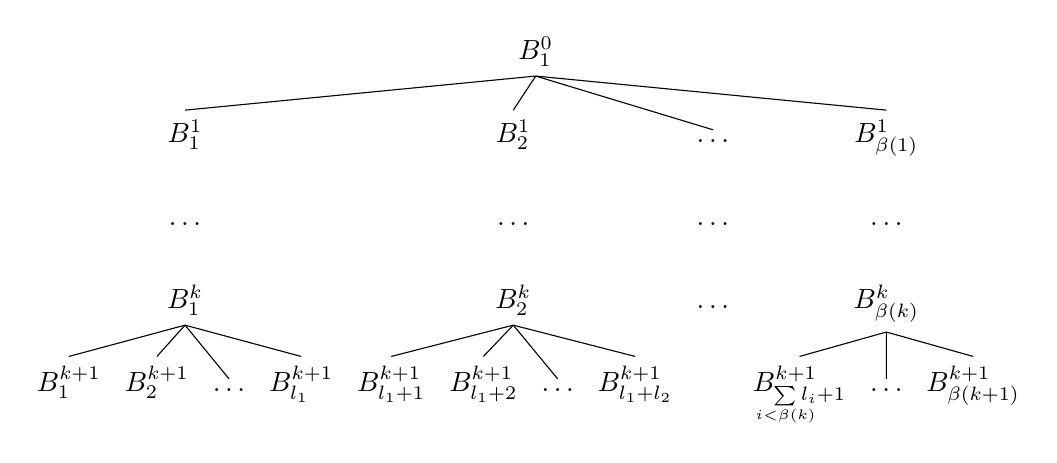
\begin{tikzpicture}
\Tree [. $B^0_1$ [. $B^1_1$ \edge [draw=none]; [. $\ldots$ \edge [draw=none]; [. $B^k_1$ [. $B^{k+1}_1$ ] [. $B^{k+1}_2$ ]  [. $\ldots$ ] [. $B^{k+1}_{l_1}$ ] ] ] ] 
		        [. $B^1_2$ \edge [draw=none]; [. $\ldots$ \edge [draw=none]; [. $B^k_2$ [. $B^{k+1}_{l_1 + 1}$ ] [. $B^{k+1}_{l_1 + 2}$ ] [. $\ldots$ ] [. $B^{k+1}_{l_1 + l_2}$ ] ] ] ] 
		        [. $\ldots$  \edge [draw=none]; [. $\ldots$ \edge [draw=none]; [. $\ldots$ ] ] ]
	                   [.$B^1_{\beta(1)}$ \edge [draw=none]; [. $\ldots$ \edge [draw=none]; [.$B^k_{\beta(k)}$ [. $B^{k+1}_{\sum\limits_{\mathclap{i < \beta(k)}}  l_i + 1 }$ ] [. $\ldots$ ] [. $B^{k+1}_{\beta(k+1)}$ ] ] ] ] ]
\end{tikzpicture}
\end{center}
\end{definition}

Before going on, first note that we have drawn $T_S$ such that leftmost child of some $B^k_i$ is $B^{k+1}_j$ where $j$ is minimal among the children of $B^k_i$, and then continued in increasing order. In general, if we draw $T_S$ so that the children of a given vertex are depicted in increasing order according to their index, then  each choice of indexing for the elements of $S_{\gamma_k}$ produces a different graphical representation of $T_S$. The structures produced by different choices of indices are clearly isomorphic as trees, and as we will see by the end of the section, each choice of indexing will be valid for our purposes as well.\\

Of central importance to us is the distance between two vertices in $T_s$. Since each vertex represents an element of $S_{\gamma_k}$, that is a closed ball in an ultrametric space, it is well-defined to let the distance between vertices be equal to the distance between a choice of centres for those balls. Note that if the distance between $B^k_i$ and $B^l_j$ is taken to be $\rho(x_i,x_j)$, for some choice of $x_i \in B^k_i$ and $x_j \in B^l_j$, say $\rho(x_i,x_j)=\gamma_n$ , then the join of  $B^k_i$ and $B^l_j$ is some $B^n_x$. 

\begin{lemma}
If $B^k_i$ and $B^l_j$ are two vertices in $T_S$, then $\rho(x_i,x_j)$, for any choice of  $x_i \in B^k_i$ and $x_j \in B^l_j$, is equal to the diameter of the join of  $B^k_i$ and $B^l_j$. 
\end{lemma}

\begin{proof}
Let $B^k_i$ and $B^l_j$ be two (distinct) vertices in $T_S$ and let $B^n_x$ be their join. The diameter of $B^n_x$ is $\gamma_n$ since $B^n_x=B(x_0, \gamma_n)$ for some $x_0$. Since $\rho$ is an ultrametric the distance between any  $x_i \in B^k_i$ and $x_j \in B^l_j$ is constant, and must be equal to the diameter of the smallest ball containing both of them, that is $\gamma_n$.
\end{proof}

In particular, we have that for any $k$ and any $i < \beta(k)$, the distances between the children of $B^k_i$ will be $\gamma_k$ and for any $i \neq j$ the distance between the children of $B^k_i$ and $B^k_j$ will be equal to the distance between  $B^k_i$ and $B^k_j$ (which will be some $\gamma_{m}, m <k$).

\section*{Recusive $\rho$-orderings}
In this section, we show how the recursive partioning of $S$ into the spaces $S_{\gamma_k}$ gives rise to a $\rho-$ordering of $S$. We first note that without loss of generality, for any $k \in \mathbb{N}$, we can reindex the $B^k_i$'s so that they give the first $\beta(k)$ terms of a $\rho_k$-ordering of $S_{\gamma_k}$, when the latter is viewed as a (finite) metric space. In the first proposition below, we note that if the $B^k_i$'s are so indexed, then finding a $\rho_{k+1}$-ordering of $S_{\gamma_{k+1}}$ is straightforward: select a $B^{k+1}_j$ from each of the $B^k_i$'s in order and then start over.  

\begin{proposition} 
Let be $S$ a compact subset of an ultrametric space $(M, \rho)$ and $\Gamma_S$, the set of distances in $S$. If $S_{\gamma_k}$ is the partition of $S$ as described above for $\gamma_k \in \Gamma_S$ with $k < \infty$, where the elements are indexed according to a $\rho_k$-ordering of $S_{\gamma_k}$, then the first $\beta(k+1)$ terms in a $\rho_{k+1}$-ordering of $S_{\gamma_{k+1}}$ can be found by selecting at each stage $n$, a child from $B^k_{\overline{n}}$, where $\overline{n} = n \mod \beta(k) +r $ and $r$ is minimal in $\{0,\ldots,\beta(k)-1\}$ such that $B^k_{n \mod \beta(k) +r}$ still has unused children.
\end{proposition}

\begin{proof}
Let $S$, $S_{\gamma_K}$, and $S_{\gamma_{k+1}}$ be as above. In particular, suppose the elements of $S_{\gamma_k}$ are indexed according to a $\rho_k-$ordering. Denote the elements of $S_{\gamma_{k+1}}$ by $B^{k+1}_{i,j}$ where the first subscript indicates that the elements is a child of $B^k_i$. To form a $\rho_{k+1}$ ordering of $S_{\gamma_{k+1}}$, we must maximize the product of distances at each step $n$.\\

Now note that $\Gamma_{S_{\gamma_k}} = \{\gamma_0, \gamma_1,\ldots, \gamma_{k-1}\}$ and $\Gamma_{S_{\gamma_{k+1}}} = \{\gamma_0, \gamma_1,\ldots, \gamma_{k-1}, \gamma_{k}\}$. That is, the distances in $S_{\gamma_{k+1}}$ are the same as the distances in $S_{\gamma_k}$, although they also include the smaller distance $\gamma_k$. Since we know that the elements $B^k_1,\ldots,B^k_{\beta(k)}$ already maximizes the product of distances in $\{\gamma_0, \gamma_1,\ldots, \gamma_{k-1}\}$, the first $\beta(k)$ terms of a $\rho_{k+1}$-ordering of $S_{k+1}$ can be found by taking $B^k_{1,j_1},\ldots, B^k_{1,j_{\beta(k)}}$ for any choice of $j$'s. At this point, any choice of next element will produce a copy of $\gamma_k$ in the $\rho_{k+1}$-sequence; however, if we chose another child of $B^k_{1}$, we are able to keep building the ordering in a canonical fashion, since we know that we will then be able to maximize the product at the next step by chosing another child of $B^k_{2}$.\\

We see then that a $\rho_{k+1}$-ordering of $S_{\gamma_{k+1}}$ is found by minimizing the number of times $\gamma_k$ is introduced into the $\rho_{k+1}$-sequence and maximizing the product among the $\gamma_0, \gamma_1,\ldots, \gamma_{k-1}$, and the latter is already known to be achieved by taking the $B^k_i$ in order.  If the $B^k_i$'s all have the same number of children, then we can always select a child of $B^k_{\overline{n}}$, where $\overline{n} = n \mod \beta(k)$ at each stage $n$, $n < \beta(k+1)$, since there will always be one available. On the other hand, suppose the $B^k_i$ have an unequal number of children and $n$ is the first step at which all the children of $B^k_{\overline{n}}$ have been exhausted. What element will maximize the $\rho_{k+1}-$sequence?\\

Consider the space $(S_{\gamma_k} \setminus B^k_{\overline{n}})$. Removal of $B^k_{\overline{n}}$ will not effect the first $m$ terms of a $\rho_k$-ordering of this space, for $m < \overline{n}$, since if a sequence of elements maximizes a function over a set $X$, they will also maximize that function of a subset of $X$ (provided they themselves remain in the subset). Then the $\rho_k-$sequence of $(S_{\gamma_k} \setminus B^k_{\overline{n}})$ begins $\{B^k_1,\ldots, B^k_{\overline{n}-1}\}$.\\

Moreover, if $B^k_{\overline{n}+1}$ maximizes $\prod^{\overline{n}}_{i=1} \rho_{k}(x, B^k_i)$ over $S_{\gamma_k}$, then it also maximizes $\prod^{\overline{n}-1}_{i=1} \rho_{k}(x, B^k_i)$ over $(S_{\gamma_k} \setminus B^k_{\overline{n}})$, since $\prod^{\overline{n}}_{i=1} \rho_{k}(x, B^k_i) = (\prod^{\overline{n}-1}_{i=1} \rho_{k}(x, B^k_i)) \cdot \rho_{k}(x, B^k_{\overline{n}})$.\\

Then the $\rho_k-$sequence of  $(S_{\gamma_k}\setminus B^k_{\overline{n}})$ is simply $\{B^k_1,\ldots, B^k_{\overline{n}-1}, B^k_{\overline{n}+1},\ldots, B^k_{\beta(k)}\}$.\\

Now we see that $\rho_{k+1}-$sequence of $S_{\gamma_{k+1}}$ is maximized by simply skipping over $B^k_{\overline{n}}$, should all its children be exhausted, and selecting a child from $B^k_{\overline{n}+1}$. Then a $\rho_{k+1}-$ordering of $S_{\gamma_{k+1}}$ is found by selecting elements of each $B^k_i$ in order as much as possible, and skipping to $B^k_{i+1}$, when it is not possible.

\end{proof}
Note that in building the $\rho_{k+1}-$ordering of $S_{\gamma_{k+1}}$ we selected, at each step, a child of some $B^k_i$, but we did not concern ourselves over which child was selected. This is because the distances between any two children of some $B^k_i$  is $\gamma_k$, and the distance between any one of them and a child of some $B^k_j$, $i \neq j$, is the same. We can now see, as claimed above, that any of the isomorphic versions of $T_ S$ are valid for producing $\rho-$orderings. Suppose then that we have created $T_s$ and (arbitrarily) indexed the children of each vertex. Then, there is no loss of genearlity in assuming that at each stage, we select a child with smallest index among its siblings, that is, that we select the leftmost available child in $T_s$. Since for ease of indexing, we will assume a $\rho-$ordering has been built by this convention, we introduce the following definition.

\begin{definition}
The $\rho-$ordering of $S$ formed by pulling elements from left to right in (a choice of) $T_s$ is call the \textbf{canonical $\rho$-ordering} of $S$ (with respect to $T_s$).
\end{definition}

The above proposition quickly leds to a recursive contruction for a $\rho-$ordering of $S$. Indeed, to build a $\rho-$ordering of $S$ from the above, it suffices only to make a choice of centres for each of $B^k_i$'s.

\begin{proposition}
Let be $S$ a compact subset of an ultrametric space $(M, \rho)$ and let $\Gamma_S$ be the set of distances in $S$. Let $S_{\gamma_k}$ be the partition of $S$ as described above for $\gamma_k \in \Gamma_S$ with $k < \infty$, where the elements are indexed according to a $\rho_k$-ordering of $S_{\gamma_k}$. Suppose each of the element of $S_{\gamma_k}$ have also been partitioned into closed balls of radius $\gamma_{k+1}$, $B^k_i =\cup_{j=1}^{l_i} B^{k+1}_{i,j}, \forall i$.\\

Let $x_{i,j}$ denote a choice of centre for the element $B^{k+1}_{i,j}$. Then the first $\beta(k+1)$ elements of a $\rho-$ordering of $S$ can be found by forming a matrix, $A_k$, whose $(i,j)^{th}$-entry is $x_{i,j}$, if $j \leq l_i$ and * otherwise, and then concatenating the rows.
\end{proposition}


\begin{proof}
The matrix $A_k$ is a representation of the $k^{th}$ and $(k+1)^{th}$ levesl of $T_S$ where the $B^k_i$'s (and $B^{k+1}_{i,j}$'s) have been replaced by a choice of centres. Since matrices must be rectangluar, the case where some $B^k_i$ and $B^k_j$ have an unequal number children is handled by inserting a placeholder, *, into $A_k$.  Moreover, since the $\rho_{k+1}$ distance between distinct closed balls is just the $\rho$ distance between a choice of centres of those  balls, a choice of centres in a $\rho_{k+1}$-ordering gives the beginning of a $\rho$-ordering.  By the above proposition, we must select elements from each $B^K_i$ one after the other, which is achieved by selecting one element from each column in order, for example by concatenating the rows (and then deleting *'s if necessary). 
\end{proof}

We get the most use out of the construction above if, in selecting a choice of centres for the $B^{k+1}_{i,j}$'s, we reuse the previous the choices as much as possible. Suppose for example we have made a choice of centres for the balls of radius $\gamma_k$ and constructed the matrix $A_{k-1}$. At the next iteration, we will need a choice of centres for the balls of radius $\gamma_{k+1}$. If $x_i$ was our choice of representative for $B^k_i$ and $x_i \in B^{k+1}_{i,j}$, we may as well let $x_i$ be our choice of representative for $B^{k+1}_{i,j}$. If we make our choice of centres in this way, then when we concatenate the rows of some $A_{k-1}$, we obtain (without loss) the first row of $A_k$. We follow this convention in the two examples below.

\begin{example}
Let us use the above to start a $\rho$-ordering of $S=(\mathbb{Z}, \lvert \cdot \rvert_3)$. We have that $\Gamma_S=\{1, \frac{1}{3},\frac{1}{9},\frac{1}{27},\ldots \}$ and $T_s$ begins:

\begin{center}
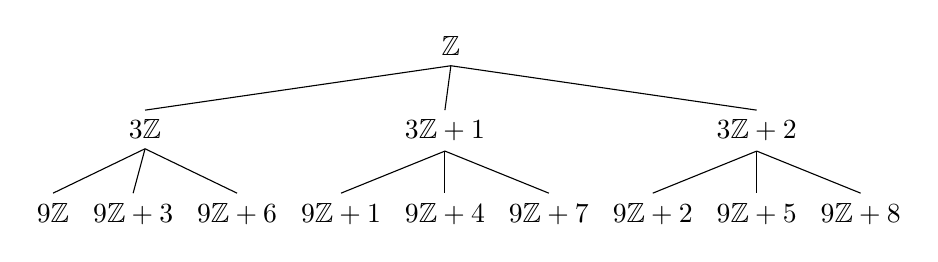
\begin{tikzpicture}
\Tree [. $\mathbb{Z}$  [. $3\mathbb{Z}$ [. $9\mathbb{Z}$ ] 
						   [. $9\mathbb{Z}+3$  ] 
						   [. $9\mathbb{Z}+6$ ] ] 
			      [. $3\mathbb{Z}+1$ [. $9\mathbb{Z}+1$ ] 
						        [. $9\mathbb{Z}+4$ ] 
						        [. $9\mathbb{Z}+7$ ] ] 
		 	      [. $3\mathbb{Z}+2$  [. $9\mathbb{Z}+2$ ] 
                                                                        [. $9\mathbb{Z}+5$ ] 
                                                                       [. $9\mathbb{Z}+8$ ] ] ] 
\end{tikzpicture}
\end{center}




We start by finding a $\rho_0$-ordering of $S_{\gamma_0}$, but this is trival since $S_{\gamma_0}$ has only a single element. Let us pick $0$ to be our choice on centre for $B^0_1=B(0,1)=\mathbb{Z}$. As we see from $T_S$, $S_{\gamma_0}$ is partitioned into $3$ closed balls of radius $\gamma_1=\frac{1}{3}$, namely $3\mathbb{Z}, 3\mathbb{Z}+1$, and $3\mathbb{Z}+2$. A choice of centres is given by $0,1$, and $2$, so that $A_0$ becomes:

\[A_0=
 \begin{pmatrix}
0 \\
1  \\
2 
\end{pmatrix}
\]


To start the $\rho-$ordering, concatenate the rows to obtain $\{0,1,2\}$, and to continue it, make a choice of centres for each of the closed balls of radius $\gamma_2=\frac{1}{9}$ partitioning the sets $3\mathbb{Z}+i$, $i \in 0,1,2$. For example, $3\mathbb{Z} =  9\mathbb{Z} \cup 9\mathbb{Z}+3 \cup 9\mathbb{Z}+6$, so a choice of centres for $B^1_1$ is given by $\{0,3,6\}$. Making choices for the remaining elements, we obtain: 

\[A_1=
 \begin{pmatrix}
0 & 1 &  2 & \\
3 & 4 &  5 & \\
6 & 7 &  8 &
\end{pmatrix}
\]

To continue the $\rho-$ordering we concatenate the rows, $\{0,1,2,3,4,5,6,7,8\}$, which also gives the first row of $A_2$. The remaining rows are found by partitioning each of the closed balls of radius $\frac{1}{9}$ and again making a choice of centres:
\[A_2=
 \begin{pmatrix}
0 & 1 &  2 & 3 & 4 & 5 & 6 & 7 & 8 \\
9 & 10 &  11 & 12 & 13 & 14 & 15 & 16 & 17 \\
18 & 19 &  20 & 21 & 22 & 23 & 24 & 25 & 26 \\
\end{pmatrix}
\]

And so on. 
\end{example}

We are able to make two statements following this example. The first is that in starting the $\rho-$ordering, the fact that $S_{\gamma_0}$ had only a single element allowed us to get started for free. In fact,  all compact ultrametric spaces are bounded, so this is always the case. \\

The second takeaway is that we found the start of a $\rho-$ordering of $S=(\mathbb{Z}, \lvert \cdot \rvert_3)$ was given by taking the integers starting at $0$ in their natural order. If we had continued building the ordering, we would have continued to find this. The fact that the natural ordering on the integers is a $\rho_p-$ordering, where $\rho_p$ is the $p-$adic metric for any prime $p$, is well known (cf. $\ldots$), but we give an alternate proof of it here: 

\begin{corollary} 
Let $S$ be the ultrametric space $(\mathbb{Z}, \rho_p)$, where $\rho_p$ is  $p-$adic metric for any prime $p$. The a $\rho_p-$ordering of $S$ can be found by taking the integers, starting at $0$, in their natural order.
\end{corollary}

\begin{proof}
We prove the above by induction on $k$. First note that for any choice of prime, the elements of $S_{\gamma_1}$ are the cosets of $\mathbb{Z}$ modulo $p$, so that $A_0$ has $p$ columns. Since $\{0,1,2\ldots,p-1\}$ are distributed among each of these cosets, without loss of generality the first row of $A_0$ is given by $[0,1,2,\ldots, p-1]$ in order.\\

Now suppose that the first row of $A_k$ is given by $[0,1,2,\ldots,n]$ for $0 \leq k < k+1$. We show the first row of $A_{k+1}$, and therefore the first $n'$ elements in a $\rho_p-$ordering of $S$, where $n'$ is the column dimension of $A_{k+1}$, can be obtained as $[0,1,2,\ldots,n,n+1,\ldots,n']$. First note that each closed ball of radius $p^k = \gamma_k$ is in fact a coset of $\mathbb{Z}$ modulo $p^k$, of which there are $p$. Then for any $k$, $A_k$ is a matrix with $p^k$ columns and $p$ rows. In particular, $n=p^k-1$. Let $i \in \{0,1,\ldots,p^{k}-1\}$ be arbitrary. Then $i$ is in exactly one of the cosets of $\mathbb{Z}$ modulo $p^k$ and since the first row of $A_k$ is $[0,1,2,\ldots,p^k-1]$, it must have been chosen as our representative of this coset. If we split $p^k\mathbb{Z}+i$ into balls of radius $p^{k+1}$, we have \[p^k\mathbb{Z}+i = \bigcup_{j=0}^{p-1} p^{k+1}\mathbb{Z} + (p^kj + i) \]
since there will be $p$ elements in the partition, each of which will be equal to $i$ modulo $p^k$ and distinct modulo $p^{k+1}$. Then, there is a choice of centres such that the $i^{th}$ column of $A_{k}$ is \[[i,p^k +i, 2p^k +i,\ldots, (p-1)p^k +i]^T\]
filling this in for each $i$, we see that $A_k$ can be obtained as:
\[A_k=
 \begin{pmatrix}
0 & 1 &  2 & \ldots & p^k -1 \\
p^k & p^k+1 &  p^k+2 & \ldots & p^k+(p^k-1) \\
2p^k & 2p^k+1 &  2p^k+2 & \ldots & 2p^k+(p^k-1) \\
\vdots &  \vdots & \vdots & \ddots & \vdots \\
(p-1)p^k & (p-1)p^k +1 &  (p-1)p^k+2 & \ldots & (p-1)p^k+(p^k-1)
\end{pmatrix}
\]

Concatenating the rows, we see the first row of $A_{k+1}$ will be \[[0,1,2,\ldots,p^k-1,p^k,\ldots,p^{k+1}-1]\] as required. 
\end{proof}

\begin{example}
Let us now see an example where there is an uneven number of children between the vertices on a given level. Suppose $S=\mathbb{Z}_{(2)} \setminus 4\mathbb{Z}$. In this case, we have that $\Gamma_S=\{1, \frac{1}{2},\frac{1}{4},\frac{1}{8},\ldots \}$ and $T_s$ begins:

\begin{center}
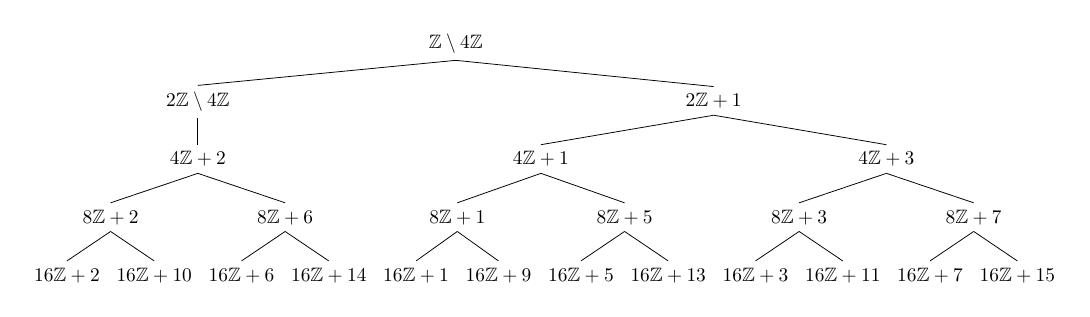
\begin{tikzpicture}[scale=.7]
\Tree [. $\mathbb{Z}\setminus 4\mathbb{Z}$  [. $2\mathbb{Z}\setminus 4\mathbb{Z}$  [. $4\mathbb{Z}+2$ [. $8\mathbb{Z}+2$ [. $16\mathbb{Z}+2$ ] [. $16\mathbb{Z}+10$ ] ] 
                                                            [. $8\mathbb{Z}+6$ [. $16\mathbb{Z}+6$ ] [. $16\mathbb{Z}+14$ ] ] ] ]
			                 [. $2\mathbb{Z}+1$ [. $4\mathbb{Z}+1$  [. $8\mathbb{Z}+1$ [. $16\mathbb{Z}+1$ ] [. $16\mathbb{Z}+9$ ] ]
			                                                        [. $8\mathbb{Z}+5$ [. $16\mathbb{Z}+5$ ] [. $16\mathbb{Z}+13$ ] ] ] 
			                                    [. $4\mathbb{Z}+3$  [. $8\mathbb{Z}+3$ [. $16\mathbb{Z}+3$ ] [. $16\mathbb{Z}+11$ ] ] 
			                                                        [. $8\mathbb{Z}+7$ [. $16\mathbb{Z}+7$ ] [. $16\mathbb{Z}+15$ ] ] ] ] ] 
\end{tikzpicture} 
\end{center}

Choosing centres for the partition of $\mathbb{Z}$ into closed balls of radius $\frac{1}{2}$, we have:
\[A_0=
 \begin{pmatrix}
2 \\
1  \\
\end{pmatrix}
\]

We have taken $S$ to be the complement of $4\mathbb{Z}$ in $\mathbb{Z}_{(2)}$, so $B(0,\gamma_1)$ has only one child, since $2\mathbb{Z} \setminus 4\mathbb{Z} = 4\mathbb{Z}+2$, while $B(1,\gamma_1)$ has two. Making a choice of centres, we have:

\[A_1=
 \begin{pmatrix}
2 & 1 \\
* & 3  \\
\end{pmatrix}
\]

We concatenate the rows, skipping over *, and again make a choice of centres for the closed balls of radius $\frac{1}{8}$:

\[A_1=
 \begin{pmatrix}
2 & 1 & 3 \\
6 & 5 & 7   \\
\end{pmatrix}
\]

One more iteration yields:

\[A_2=
 \begin{pmatrix}
2 & 1 & 3 & 6 & 5 & 7 \\
10 & 9 & 11 & 14 & 13 & 15   \\
\end{pmatrix}
\]

So that a $\rho_2-$ordering of $S=\mathbb{Z}_{(2)} \setminus 4\mathbb{Z}$ starts: $\{2,1,3,6,5,7,10,9,11,14,13,15,\ldots\}$.

\end{example}


%\begin{corollary}
%Interweaving the bottom row of the lattice of closed balls for a set $S$ gives a $\rho$-ordering of $S$. 
%\end{corollary}
In the two propositions above, there was notational difficulty that arose when there was an unequal number of children between the vertices on a given level of $T_s$. This difficulty is, in fact, more than a notational inconvenience, and the situation simplifies considerably when it is not the case. We are far from the first to observe this. Amice noted this as far back as her 1964 paper, and it has been observed more recently in several papers by Fares and colleagues. The following section discusses this in more detail, first by supplying some preliminary lemmas and then showing how calculations are simplified in this setting.

\section*{Semi-regularity}
In this section, we restrict to the case where in the tree $T_s$, for $S$ some compact subset of an ultrametric space, every vertex on a given level has the same number of children. In this case, we can attach another sequence to $S$, which we call the $\alpha-$sequence of $S$ and which describes, for each level $k \in \mathbb{N}$, the size of the partitions on that level. We develop some preliminary lemmas, which we then use to derive formulae for this special case.

\begin{definition}
Let $S$ be as above, a compact subset of an ultrametric space $(M, \rho)$. We say that $S$ is \textbf{semi-regular} if $T_{B^k_i} \cong T_{B^k_j}$, $\forall k \in \mathbb{N}$ and  $i,j \in \beta(k)$, and where the isomorphism is understood as an isomorphism of trees. That is, $S$ is semi-regular if each ball of radius $\gamma_k$ breaks into the same number of balls of radius $\gamma_{k+1}$, for all $k$. If there exists an $n \in \mathbb{N}$ such that $T_{B^N_i} \cong T_{B^N_j}$ for all $N \geq n$, i.e.  each ball of radius $\gamma_N$ breaks into the same number of balls of radius $\gamma_{N+1}$ for $N \geq n$, then we say $S$ is \textbf{eventually semi-regular}.
\end{definition}

\begin{definition}
Suppose $S$ is a compact subset of an ultrametric space and $S$ is semi-regular. The \textbf{$\alpha$-sequence} of $S$ is the sequence given by $\alpha(k)=\frac{\beta(k+1)}{\beta(k)}$, which is in $\mathbb{N}$ for each $k$. That is, if $B^k_i$ is an element of $S_{\gamma_k}$, then $\alpha(k)$ is equal to the number of children of $B^k_i$ in $T_s$. Since $S$ is semi-regular, this number does not depend on $i$.
\end{definition}


\begin{lemma}
$\lfloor\frac{n}{q} \rfloor$ counts the numbers strictly less than $n$ that are congruent to $n \mod q$.
\end{lemma}

\begin{proof}
(sketch) Every multiple of $q$ produces exactly one of the numbers from $1$ to $q$ and exactly one of those is the residue class of $n$ modulo $q$. The remainder is the residue class of $n$ itself and since we only want the numbers strictly less than $n$, we ignore this by taking the floor.
\end{proof}


\begin{lemma}
\[\lfloor\frac{n}{b} \rfloor - \lfloor \frac{n}{ab} \rfloor = \sum_{k=1}^{a-1} \lfloor \frac{n + kb}{ab} \rfloor\] for $n,a,b \in \mathbb{N}$. In particular, 
\[\lfloor\frac{n}{b} \rfloor - \lfloor \frac{n}{2b} \rfloor= \lfloor \frac{n+b}{2b} \rfloor\] for  $n,b \in \mathbb{N}$.
\end{lemma}

\begin{proof}
\[\lfloor\frac{n}{b} \rfloor - \lfloor \frac{n}{ab} \rfloor = \lfloor a \cdot \frac{n}{ab} \rfloor - \lfloor \frac{n}{ab} \rfloor  = \sum_{k=0}^{a-1} \lfloor \frac{n}{ab} + \frac{k}{a} \rfloor - \lfloor \frac{n}{ab} \rfloor \text{ (*)}\]
\[= \sum_{k=1}^{a-1} \lfloor \frac{n}{ab} + \frac{k}{a} \rfloor = \sum_{k=1}^{a-1} \lfloor \frac{n + kb}{ab} \rfloor \]
where the final step in (*) is due to Hermite's identity: $\lfloor nx \rfloor = \sum_{k=0}^{n-1} \lfloor x + \frac{k}{n} \rfloor$, for $n \in \mathbb{N}$ and $x \in \mathbb{R}$.
\end{proof}                                                                                                              

\begin{lemma}
If $S$ is semi-regular and $\delta$ denotes the canonical $\rho$-ordering of $S$, that is, a $\rho-$ordering formed by pulling from left to right in $T_s$, then \[\rho(\delta(n),\delta(m))=\gamma_k\] if, and only if, \[ n=m \mod \beta(k) \text{  and } n \neq m \mod \beta(k+1)\]
\end{lemma}

\begin{proof}
Since $S$ is semi-regular, every sequence of $\beta(k)$ terms in $\delta$ will be from each of distinct elements of $S_{\gamma_k}$ (for any $k$). Moreover, since $\delta$ is a canonical $\rho-$ordering, we always pull from the elements of $S_{\gamma_k}$ in the same order. Then $\delta(n)$ and $\delta(m)$ are descendents of some $B^k_j$ if, and only if, $n = m \mod \beta(k)$. Then the result follows since $\rho(\delta(n),\delta(m))=\gamma_k$ if, and only if, $B^k_i$ for some $i \in 1,\ldots, \beta(k)$ is the join of $B^n_i \ni \delta(n)$ and $B^m_{i'} \ni \delta(m)$.  \\ 
\end{proof}


\begin{proposition}
If $S$ is a semi-regular ultrametric space, $\sigma$ is the characteristic sequence of $S$, $\beta$ is the structure sequence of $S$, and $\alpha$ is the sequence describing the semi-regularity, then
\[v_{\gamma_k}(\sigma(n)) =  \lfloor\frac{n}{\beta(k)}\rfloor - \lfloor\frac{n}{\beta(k+1)}\rfloor = \sum_{j=1}^{\alpha(k)-1} \lfloor \frac{n + j\cdot \beta(k)}{\alpha(k)\beta(k)} \rfloor\]
\end{proposition}

\begin{proof}
The exponent of $\gamma_k$ in the $n^{th}$ term of the characteristic sequence is the number of $m$ strictly less than $n$ such that $\rho(\sigma(n),\sigma(m))=\gamma_k$. By the lemma above, this the number of $m <n$ such that $m = n \mod \beta(k)$  and $m \neq n \mod \beta(k+1)$, which by the previous lemma is $\lfloor\frac{n}{\beta(k)}\rfloor - \lfloor\frac{n}{\beta(k+1)}\rfloor$. Then we have:
\begin{flalign*}
 v_{\gamma_k}(\sigma(n)) & \\
 = \lfloor\frac{n}{\beta(k)}\rfloor - \lfloor\frac{n}{\beta(k+1)}\rfloor & \\
 = \lfloor\frac{n}{\beta(k)}\rfloor - \lfloor\frac{n}{\beta(k)\alpha(k)}\rfloor\text{,} & \text{ because } S \text{ is semi-regular}\\
 = \sum_{j=1}^{\alpha(k)-1} \lfloor \frac{n + j\cdot \beta(k)}{\alpha(k)\beta(k)} \rfloor
\end{flalign*}
\end{proof}



\begin{example}
Consider the ultrametric space $(\mathbb{Z}, \rvert \cdot \lvert_p)$  for any prime $p$. Then $\beta(k)=p^k$ and $\alpha(k)=p$ for any $k$. The above gives 
\[v_{\gamma_k}(\sigma(n)) =\lfloor \frac{n}{p^{k}}\rfloor - \lfloor \frac{n}{p^{k+1}} \rfloor\]
and since $\gamma_k = p^{-k}$, $\forall k$, we have 
\[v_{\frac{1}{p}}(\sigma(n)) \]
\[ = \sum_{k=1}^{\infty} k \cdot (\lfloor \frac{n}{p^{k}}\rfloor - \lfloor \frac{n}{p^{k+1}} \rfloor) \]
\[ = \sum_{k=1}^{\lceil log_p(n) \rceil}  k \cdot (\lfloor \frac{n}{p^{k}}\rfloor - \lfloor \frac{n}{p^{k+1}} \rfloor)\]
\[ = \lfloor \frac{n}{p}\rfloor - \lfloor \frac{n}{p^{2}} \rfloor +  2\lfloor \frac{n}{p^2}\rfloor - 2\lfloor \frac{n}{p^3} \rfloor + \ldots +  \lceil log_p(n)\rceil \lfloor \frac{n}{p^{ \lceil log_p(n)\rceil}} \rfloor \]
\[ = \lfloor \frac{n}{p}\rfloor + \lfloor \frac{n}{p^2}\rfloor  + \ldots +  \lfloor \frac{n}{p^{ \lceil log_p(n)\rceil}} \rfloor \]
\[ =  \sum_{k=1}^{\lceil log_p(n) \rceil} \lfloor \frac{n}{p^{k}}\rfloor \]
\[ =  \sum_{k=1}^{\infty} \lfloor \frac{n}{p^{k}}\rfloor \]
\[= v_{p}(n!) \]

since $\lfloor \frac{n}{p^k} \rfloor = 0$ if $ p^k > n \iff log(p^k) > log(n) \iff k > log_p(n)$, so that we are able to recover the well-known Legendre's formula.
\end{example}

Some comment about how the above starts to build up a toolkit independent of  algebraic structure in $S$.

\begin{corollary}
If $G$ is a compact ultrametric group, then $G$  is semi-regular.
\end{corollary}

\begin{proof}
Since $G$ is a group, each ball centred at $0$ is in fact a subgroup of $G$. Then each set of elements of $S_{\gamma_k}$ is a collection of cosets of $G/B(0,\gamma_k)$. Since $G$ is assumed to be compact, $G/B(0,\gamma_k)$ is finite and so Lagrange's theorem implies the result.
\end{proof}

Semi-regularity gives a notion of translation invariance to ultrametric spaces that are not themselves groups. In the previous section, we observed that spaces which admitted both translation invariance and scaling had valuative capacity that could be computed explicity via the subadditivity formula. Is there a way to define this for ultrametric which are not normed vector spaces?

\begin{definition}
Let $S$ be a semi-regular compact subset of an ultrametric space. If there exists a $q \in \mathbb{N}$ such that $\alpha(n) = q$, for all $n$, then $S$ is said to be \textbf{regular}. If there exists a $q \text{ and } N$ in $\mathbb{N}$ such that $\alpha(n) = q$, for all $n \geq N$, then $S$ is said to be $\textbf{eventually regular}$.
\end{definition}

Alt.:
\begin{definition}
Let $S$ be a semi-regular compact subset of an ultrametric space. If there exists a $q_1,\ldots,q_m \in \mathbb{N}$ such that $\alpha(n) = q_i$ if, and only if, $n = i \mod m$, that is, $\alpha$ has an infinitely-repeating finite subsequence of length $m$, then we say $S$ is $\textbf{periodic}$. If $m=1$, then $S$ is $\textbf{regular}$. 
\end{definition}

$S$ is regular just in case the $\alpha-$sequence of $S$ is constant. In what follows, we assume that $S$ is regular, but the results carry over to the case where $S$ is peroidic with the obvious adjustments. To make use of regularity in $S$ we should, before continuing, also put some constraints on our sequence of distances $\Gamma_S$.

\begin{definition}
Let $S$ be a compact subset of an ultrametric space and $\Gamma_S$ is the sequence of decreasing distances in $S$. Then we say $S$ is \textbf{well-behaved} (I guess - or tame? reasonable?), if $S$ is semi-regular and $\gamma_k = \alpha(k)^{c_k}$ for all $k \in \mathbb{N}$ and some $c_k \in \mathbb{Z}$.
\end{definition}

\begin{example}
Any ultrametric space where $\rho$ is induced from a valuation domain.
\end{example}

If $S$ is regular with $\alpha(k)=q$, for all $k$:
\[v_{\gamma_k}(\sigma(n)) =  \lfloor\frac{n}{q^k}\rfloor - \lfloor\frac{n}{q^{k+1}}\rfloor \]
\[v_{q^{c_k}}(\sigma(n)) =  \lfloor\frac{n}{q^k}\rfloor - \lfloor\frac{n}{q^{k+1}}\rfloor \]
\[v_{q}(\sigma(n)) =  \sum_{k=0}^{\infty} c_k \cdot(\lfloor\frac{n}{q^k}\rfloor - \lfloor\frac{n}{q^{k+1}}\rfloor) \]
\[v_{q}(\sigma(n)) =  \sum_{k=0}^{\lceil log_q(n) \rceil} c_k \cdot(\lfloor\frac{n}{q^k}\rfloor - \lfloor\frac{n}{q^{k+1}}\rfloor) \]
\[=  c_0{n} - c_0\lfloor\frac{n}{q}\rfloor + c_1\lfloor\frac{n}{q}\rfloor - c_1\lfloor\frac{n}{q^{2}}\rfloor  + c_2\lfloor\frac{n}{q^2}\rfloor - c_2\lfloor\frac{n}{q^{3}}\rfloor \ldots + \lceil log_q(n) \rceil \lfloor\frac{n}{q^{\lceil log_q(n) \rceil}}\rfloor - \lceil log_q(n) \rceil\lfloor\frac{n}{q^{\lceil log_q(n) \rceil}}\rfloor  \]
\[v_{q}(\sigma(n)) =  \sum_{k=0}^{\lceil log_q(n) \rceil} (c_{k+1} - c_k) \cdot(\lfloor\frac{n}{q^{k+1}}\rfloor) \]

Note that the coefficient $ (c_{k+1} - c_k)$  is always positive: since $\Gamma$ is (strictly) decreasing and $\gamma_k=q^{c_k}$, the sequence $c_k$ is  also be strictly descreasing (since $\gamma_k=q^{c_k}$ implies $log_q(\gamma_k)=c_k$ and log is a monotone function). The above implies that:

\[\omega(S) = \lim_{n\to\infty} \sum_{k=0}^{\lceil log_q(n) \rceil} (c_{k+1} - c_k) \cdot(\lfloor\frac{n}{q^{k+1}}\rfloor)\]

%\begin{corollary}
%If $S$ is a (eventually) semi-regular ultrametric space and the $\alpha$ sequence of $S$ is (eventually)  periodic, then the valuative capacity of $S$ is algebraic.
%\end{corollary}

%\begin{corollary}
%Suppose $S$ and $T$ are compact subsets of an ultrametric space $M$ with $\Gamma_S = \Gamma_T$ and $\mid S_{\gamma_k}\mid =\mid T_{\gamma_k}\mid$, $\forall k$. Then $\omega(S) = \omega(T)$. 
%\end{corollary}
%\begin{itemize}
%\item i think this coincides with translation invariance when there is a group operation
%\end{itemize}


%Semi-regularity in $S$ reflects horizontal similarity on every level of $T_S$, and so we expect semi-regularity to simplify the calculation of valuative capacity.

%\begin{proposition}
%Let $S$ be a semi-regular, compact subset of an ultrametric space. Let $\Gamma_S$ be the set of distances in $S$ and let $B$ be the first element of $S_{\gamma_1}$. Let $\sigma^S(i)$  be the characteristic sequence of $S$ and $\sigma^B(i)$ be the characteristic sequence of $B$. Then,

%\[\sigma^S(\beta(0) \cdot n)=\gamma_0^c \cdot \sigma^{B}(n)\]

%where $c$ counts the numbers in $1$ to $\beta(0) \cdot n$ that are not divisible by $\beta(0)$.

%\end{proposition}

%\begin{proof}
%(sketch)
%If $n=0$, then $c=0$ and $\beta(0) \cdot n = 0$, and,
%\[\sigma^S(0)= 1 =	1 \cdot \sigma^{B}(0)\]
%since the $0^{th}$-term of any characteristic sequence is $1$ by definition. When $n=1$, $c=\beta(0)-1$, so that the right-hand side becomes,
%\[\gamma_0^{\beta(0)-1} \cdot \sigma^{B}(1)\]
%Now note that the $\beta(0)^{th}$ term of $\sigma^S$ will have $\beta(0)-1$ copies of $\gamma_0$ (one from each of the elements of $S_{\gamma_0}$ not containing the $\beta(0)^{th}$ element) and the remaining term is in the branch $B$, so it is given by $\sigma^B(1)$, and so,
%\[\sigma^S(\beta(0))=\gamma_0^{\beta(0)-1} \cdot \sigma^{B}(1)\]


%Suppose:
%\[\sigma^S(\beta(0) \cdot n)=\gamma_0^{c_n} \cdot \sigma^{B}(n)\]

%for $0 \leq n < n +1$ and consider $\sigma^S(\beta(0) \cdot (n+1))$. $\sigma^S(\beta(0) \cdot (n+1))$ will add $\beta(0)$ more terms to $\sigma^S(\beta(0) \cdot n)$. Moreover, exactly $\beta(0)-1$ of these additional terms will be in other branches and $1$ term will be in $B$, since any sequence of $\beta(0)$ terms in the $\rho-$ordering of $S$ will be from each of the $\beta(0)$ branches. Each of the $\beta(0)-1$ terms from other branches will add a copy of $\gamma_0$ and remaining term can be found by looking ahead in $\sigma^B$, so that

%\begin{align*}
%\sigma^S(\beta(0) \cdot (n+1)) && \\
%= \sigma^S(\beta(0) \cdot n) \cdot \gamma_0^{\beta(0)-1} \cdot \frac{\sigma^B(n+1)}{\sigma^B(n)} && \\
%= {\gamma_0^{c_n}} \cdot \sigma^{B}(n) \cdot \gamma_0^{\beta(0)-1} \cdot  \frac{\sigma^B(n+1)}{\sigma^B(n)} &&\\
%= {\gamma_0^{c_n}}  \cdot \gamma_0^{\beta(0)-1} \cdot  \sigma^B(n+1) && \\
%= {\gamma_0^{c_{n+1}}} \cdot  \sigma^B(n+1) 
%\end{align*}

%\end{proof}
%Since semi-regularity requires horizontal similarity at every level of $T_S$, we can repeat the branch cuts as many times as needed to calculate $\sigma(n)$.


\chapter{The structure of $T_S$}
In the previous chapter, we explored in detail the final Corollary of Chapter 2. This corollary lead us to study the lattice of closed balls in $S$, which we called $T_S$. In this chapter, we take what we have learned and explore the preceding Corollary, repeated below.\\

\begin{corollary*}
	Suppose $S = \cup_i^n S_i$ with $\rho(S_i, S_j)=d=diam(S)$ and also $\omega(S_i)=\omega(S_j)$, $\forall i,j$.  Let $r \in \mathbb{R}$ be such that $\omega(S_i)=r\omega(S)$, $\forall i$. Then $\omega(S) = r^{\frac{1}{n-1}}$. 
\end{corollary*}

In particular, we seek answers to the following questions: when does such a partition of $S$ exist and given such a partition, when are we able to compute the scaling factor $r$? In doing so, we show that the structure of $T_S$ plays an important role. 


\section{Semi-regularity}
In this section, we restrict to the case where in the tree $T_s$, for $S$ a compact, discretely-valued subset of an ultrametric space, every vertex on a given level has the same number of children. In this case, we can attach another sequence to $S$, which we call the $\alpha-$sequence of $S$ and which describes, for each level $k \in \mathbb{N}$, the size of the partitions on that level. We develop some preliminary lemmas, which we then use to derive formulae for this special case. This situation corresponds to what previous authors (\cite{amice}, \cite{cef}, \cite{fp}) have called \textit{regularity}, a term which we reserve for the next section. \\

In the definitions that follow, we recall that the $\beta-$sequence of $S$ counts the number of elements of $S_{\gamma_k}$.\\


\begin{definition}
Let $S$ be as before, a compact, discretely-valued subset of an ultrametric space $(M, \rho)$. We say that $S$ is \textbf{semi-regular} if $T_{B^k_i} \cong T_{B^k_j}$, $\forall k \in \mathbb{N}$ and  $i,j \in \beta(k)$, and where the isomorphism is understood as an isomorphism of trees. That is, $S$ is semi-regular if each ball of radius $\gamma_k$ breaks into the same number of balls of radius $\gamma_{k+1}$, for all $k$. If there exists an $n \in \mathbb{N}$ such that $T_{B^N_i} \cong T_{B^N_j}$ for all $N \geq n$, that is,  each ball of radius $\gamma_N$ breaks into the same number of balls of radius $\gamma_{N+1}$ for $N \geq n$, then we say $S$ is \textbf{eventually semi-regular}.
\end{definition}


\begin{definition}
Suppose $S$ is a compact, discretely-valued subset of an ultrametric space and $S$ is semi-regular. The \textbf{$\alpha$-sequence} of $S$ is the sequence given by \[\alpha(k)=\frac{\beta(k+1)}{\beta(k)}\] which is in $\mathbb{N}$ for each $k$. That is, if $B^k_i$ is any element of $S_{\gamma_k}$, then $\alpha(k)$ is equal to the number of children of $B^k_i$ in $T_s$. Since $S$ is semi-regular, this number does not depend on $i$.
\end{definition}

\begin{example}
\label{lagrange}	
	If $G$ is a compact ultrametric space and also a group, each ball centred at $0$ is in fact a subgroup of $G$. Then each set of elements of $S_{\gamma_k}$ is a collection of cosets of $G/B(0,\gamma_k)$. Since $G$ is assumed to be compact, $G/B(0,\gamma_k)$ is finite and so Lagrange's theorem implies that $G$ is semi-regular.
\end{example}

We now work towards a formula for the terms in the $\rho-$sequence of a semi-regular space $S$. We need a few lemmas to get started.\\
 
\begin{lemma}
Let $n$ and $q$ be in $\mathbb{N}$. Then $\lfloor\frac{n}{q} \rfloor$ counts the numbers in $\{0,\ldots, n-1\}$ that are congruent to $n \mod q$.
\end{lemma}

\begin{proof}
By the division algorithm, we know there exists unique $c,r \in \mathbb{Z}$ such that \[n = cq + r\] with $0 \leq r < q$. Since $c$ counts the number of $q$-multiples in the set $\{1,\ldots,n\}$, and each $q$-multiple contains exactly one element that is congruent to $n \mod q$, we need only show $\lfloor\frac{n}{q} \rfloor = c$. Simply note that the above implies  \[\frac{n}{q} = c + \frac{r}{q}\] and we must have   $\frac{r}{q} < 1$. Then $c$ is the largest integer such that $\frac{n}{q} \leq c$, but this is the definition of $\lfloor\frac{n}{q} \rfloor$.
\end{proof}


\begin{lemma}
\label{semi-regular formula}
\[\lfloor\frac{n}{b} \rfloor - \lfloor \frac{n}{ab} \rfloor = \sum_{k=1}^{a-1} \lfloor \frac{n + kb}{ab} \rfloor\] for $n,a,b \in \mathbb{N}$. In particular, 
\[\lfloor\frac{n}{b} \rfloor - \lfloor \frac{n}{2b} \rfloor= \lfloor \frac{n+b}{2b} \rfloor\] for  $n,b \in \mathbb{N}$.
\end{lemma}

\begin{proof}
\[\lfloor\frac{n}{b} \rfloor - \lfloor \frac{n}{ab} \rfloor = \lfloor a \cdot \frac{n}{ab} \rfloor - \lfloor \frac{n}{ab} \rfloor  = \sum_{k=0}^{a-1} \lfloor \frac{n}{ab} + \frac{k}{a} \rfloor - \lfloor \frac{n}{ab} \rfloor \text{ (*)}\]
\[= \sum_{k=1}^{a-1} \lfloor \frac{n}{ab} + \frac{k}{a} \rfloor = \sum_{k=1}^{a-1} \lfloor \frac{n + kb}{ab} \rfloor \]
where the final step in (*) is due to Hermite's identity: $\lfloor nx \rfloor = \sum_{k=0}^{n-1} \lfloor x + \frac{k}{n} \rfloor$, for $n \in \mathbb{N}$ and $x \in \mathbb{R}$.
\end{proof}                                                                                                              

\begin{lemma}
If $S$ is semi-regular and $\sigma$ denotes the canonical $\rho$-ordering of $S$, that is, a $\rho-$ordering formed by pulling from left to right in $T_s$, then \[\rho(\sigma(n),\sigma(m))=\gamma_k\] if and only if \[ n \equiv m \mod \beta(k) \text{  and } n \not\equiv m \mod \beta(k+1)\]
\end{lemma}

\begin{proof}
Since $S$ is semi-regular, every sequence of $\beta(k)$ terms in $\sigma$ will be from each of the distinct elements of $S_{\gamma_k}$ (for any $k$). Moreover, since $\sigma$ is a canonical $\rho-$ordering, we always pull from the elements of $S_{\gamma_k}$ in the same order. Then $\sigma(n)$ and $\sigma(m)$ are descendents of some $B^k_j$ if and only if $n = m \mod \beta(k)$. Then the result follows since $\rho(\sigma(n),\sigma(m))=\gamma_k$ if and only if $B^k_i$ for some $i \in 1,\ldots, \beta(k)$ is the join of $B^{k'}_i \ni \sigma(n)$ and $B^{k'}_{i'} \ni \sigma(m)$.  \\ 
\end{proof}

We introduce another piece of notation before continuing.

\begin{notation}
	Let $S$ be a compact, discretely-valued subset of an ultrametric space, $\Gamma_S$ the set of distances in $S$ and $\delta(n)$ the characteristic sequence of $S$. Suppose $\gamma_k$ is an element of $\Gamma_S$. Then we denote by $v_{\gamma_k}(\delta(n))$ the exponent of $\gamma_k$ in the $n^{th}-$term of the characteristic sequence of $S$.
\end{notation}

\begin{proposition}
If $S$ is a semi-regular ultrametric space, $\delta$ is the characteristic sequence of $S$, $\beta$ is the structure sequence of $S$, and $\alpha$ is the sequence describing the semi-regularity, then
\[v_{\gamma_k}(\delta(n)) =  \lfloor\frac{n}{\beta(k)}\rfloor - \lfloor\frac{n}{\beta(k+1)}\rfloor = \sum_{j=1}^{\alpha(k)-1} \lfloor \frac{n + j\cdot \beta(k)}{\alpha(k)\beta(k)} \rfloor\]
\end{proposition}

\begin{proof}
The exponent of $\gamma_k$ in the $n^{th}$ term of the characteristic sequence is the number of $m$ strictly less than $n$ such that $\rho(\delta(n),\delta(m))=\gamma_k$. By Lemma 7, this is the number of $m <n$ such that $m = n \mod \beta(k)$  and $m \neq n \mod \beta(k+1)$, which by Lemma 5 is $\lfloor\frac{n}{\beta(k)}\rfloor - \lfloor\frac{n}{\beta(k+1)}\rfloor$. Then we have:
\begin{flalign*}
 v_{\gamma_k}(\delta(n)) & \\
 = \lfloor\frac{n}{\beta(k)}\rfloor - \lfloor\frac{n}{\beta(k+1)}\rfloor & \\
 = \lfloor\frac{n}{\beta(k)}\rfloor - \lfloor\frac{n}{\beta(k)\alpha(k)}\rfloor\text{,} & \text{ because } S \text{ is semi-regular}\\
 = \sum_{j=1}^{\alpha(k)-1} \lfloor \frac{n + j\cdot \beta(k)}{\alpha(k)\beta(k)} \rfloor
\end{flalign*}
\end{proof}



\begin{example}
\label{legendre}
Consider the ultrametric space $(\mathbb{Z}, \rho_p)$  for any prime $p$. Then $\beta(k)=p^k$ and $\alpha(k)=p$ for any $k \in \mathbb{N} \cup 0$. Proposition 25 gives \\ \newpage
\[v_{\gamma_k}(\delta(n)) =\lfloor \frac{n}{p^{k}}\rfloor - \lfloor \frac{n}{p^{k+1}} \rfloor\]
Now since $\gamma_k = p^{-k}$, $\forall k$, we are able to compute the exponent of $\frac{1}{p}$ in $\delta(n)$. We have 
\[v_{\frac{1}{p}}(\delta(n)) \]
\[ = \sum_{k=1}^{\infty} k \cdot (\lfloor \frac{n}{p^{k}}\rfloor - \lfloor \frac{n}{p^{k+1}} \rfloor) \]
\[ = \sum_{k=1}^{\lceil \log_p(n) \rceil}  k \cdot (\lfloor \frac{n}{p^{k}}\rfloor - \lfloor \frac{n}{p^{k+1}} \rfloor)\]
\[ = \lfloor \frac{n}{p}\rfloor - \lfloor \frac{n}{p^{2}} \rfloor +  2\lfloor \frac{n}{p^2}\rfloor - 2\lfloor \frac{n}{p^3} \rfloor + \ldots +  \lceil \log_p(n)\rceil \lfloor \frac{n}{p^{ \lceil \log_p(n)\rceil}} \rfloor \]
\[ = \lfloor \frac{n}{p}\rfloor + \lfloor \frac{n}{p^2}\rfloor  + \ldots +  \lfloor \frac{n}{p^{ \lceil \log_p(n)\rceil}} \rfloor \]
\[ =  \sum_{k=1}^{\lceil log_p(n) \rceil} \lfloor \frac{n}{p^{k}}\rfloor \]
\[ =  \sum_{k=1}^{\infty} \lfloor \frac{n}{p^{k}}\rfloor \]

We are able to simplify to a finite sum in the above because $\lfloor \frac{n}{p^k} \rfloor = 0$ if \[ p^k > n \iff \log(p^k) > \log(n) \iff k > log_p(n)\]
We have already seen that the natural order on the integers gives a $\rho_p$-ordering for each $p$. So then \[\sum_{k=1}^{\infty} \lfloor \frac{n}{p^{k}}\rfloor= v_{\frac{1}{p}}(\delta(n)) = v_{\frac{1}{p}}(\prod_{i=0}^n \frac{1}{p}^{v_p(n-i)}) = \sum_{i=0}^{n-1} v_p(n-i)= v_{p}(n!)  \]
so that we are able to recover the well-known Legendre's formula.\\
\end{example}

We end this section with the following observation.

\begin{proposition}
	Let $S$ be a semi-regular subset of an ultrametric space $(M,\rho)$. Let $S_{\gamma_1}$ be the partition of $S$ described in chapter $3$, that is,
	\[S_{\gamma_1} = \bigcup_{i=1}^{n} B(x_i,\gamma_1) = \bigcup_{i=1}^{n} B^1_i\]
	Then $\rho(B^1_i, B^1_j) = d = diam(S)$ for any $i \neq j$ in $1,\ldots,n$ and $\omega( B^1_i) = \omega( B^1_j)$ for all $i$ and $j$.
\end{proposition}

\begin{proof}
	The fact that  $\rho(B^1_i, B^1_j) = d = diam(S)$ for any $i \neq j$ is clear and does not depend on the fact that $S$ is semi-regular. In fact, there are plently of ways to see this, but for example, we simply note $\rho(B^1_i, B^1_j) \in \Gamma_S$  and $ \gamma_1 < \rho(B^1_i, B^1_j)\leq \gamma_0 = diam(S)$.\\
	
	To see that $\omega( B^1_i) = \omega( B^1_j)$, we note that since $S$ is semi-regular, each $B^1_i$ is semi-regular as well. Moreover, since $S$ is semi-regular, the $\beta$ sequences of $B^1_i$ and $B^1_j$ are the same for each $i$ and $j$. Then the result follows: let $\delta^{B^1_i}(n)$ and $\delta^{B^1_j}(n)$ be the characteristic sequences of $B^1_i$ and $B^1_j$ respectively. We see that for all $k$,
	  
	  \[v_{\gamma_k}(\delta^{B^1_i}(n)) =  \lfloor\frac{n}{\beta^B(k)}\rfloor - \lfloor\frac{n}{\beta^B(k+1)}\rfloor =  v_{\gamma_k}(\delta^{B^1_j}(n)) \]
	where $\beta^B(k)$ is the $\beta$ sequence for each  $B^1_i$.
	 
\end{proof}

Now we have one answer to our first question: when $S$ is semi-regular, we can use the elements of $S_{\gamma_1}$ to build the partition from Corollary 3. The content of that corollary gave a formula for the valuative capacity. Then if $S$ is semi-regular, the principal obstacle to computing the capacity of $S$ is the identification of the scaling factor. This leads to our second question: when can we compute $r$?

\section{Regularity}
In Example \ref{legendre}, the fact that we were able to reduce to a finite sum was not the only reason we were able to simplify the calculations. It also helped a great deal that the sum was telescoping. What does the fact that we saw a telescoping sum have to do with computing the scaling factor $r$? We explore the inter-relatedness of these situations, and with the definition below, in this section.

\begin{definition}
Let $S$ be a semi-regular subset of an ultrametric space. If there exists a $q \in \mathbb{N}$ such that $\alpha(n) = q$, for all $n$, then $S$ is said to be \textbf{regular}\footnote{This is non-standard: what previous authors (\cite{amice},\cite{cef}, \cite{fp}) have called regular is what we have called semi-regular. Note that $S$ is regular in the present sense if and only if $T_S$ is regular in the standard graph theory terminology.}. %If there exists a $q \text{ and } N$ in $\mathbb{N}$ such that $\alpha(n) = q$, for all $n \geq N$, then $S$ is said to be $\textbf{eventually regular}$.
\end{definition}

%Alt:
%\begin{definition}
%Let $S$ be a semi-regular compact subset of an ultrametric space. If there exists a $q_1,\ldots,q_m \in \mathbb{N}$ such that $\alpha(n) = q_i$ if, and only if, $n = i \mod m$, that is, $\alpha$ has an infinitely-repeating finite subsequence of length $m$, then we say $S$ is $\textbf{periodic}$. If $m=1$, then $S$ is $\textbf{regular}$. 
%\end{definition}

So then $S$ is regular just in case $S$ is semi-regular and the $\alpha-$sequence of $S$ is constant. We need to make one more definition before we begin calculations. \\

\begin{definition}
Let $S$ be a semi-regular subset of an ultrametric space and $\Gamma_S$ the sequence of decreasing distances in $S$. Then we say $S$ is \textbf{tame}, if for $\gamma_k \in \Gamma_S$, \[\gamma_k = \alpha(k)^{c_k}\] for some $c_k \in \mathbb{Q}$ and for all $k \in \mathbb{N}$.
\end{definition}

Now we see what this situation means for calculations.\\

\begin{proposition}
	Let $S$ be a regular, tame subset of a compact ultrametric space with $\gamma_k = q^{c_k}$ for some $c_k \in \mathbb{Q}$ and for all $k \in \mathbb{N} \cup 0$. Then 
	\[v_{q}(\delta(n)) =  c_0n + \sum_{k=1}^{\infty} (c_{k} - c_{k-1}) \cdot \lfloor\frac{n}{q^{k}}\rfloor \]
	 and 
	\[\log_q(\omega(S)) = \lim_{n\to\infty} c_0 + \frac{1}{n}\sum_{k=1}^{\infty} (c_{k} - c_{k-1}) \cdot \lfloor\frac{n}{q^{k}}\rfloor  \]
\end{proposition}

\begin{proof}
	We know that,
\[v_{\gamma_k}(\delta(n)) =  \lfloor\frac{n}{q^k}\rfloor - \lfloor\frac{n}{q^{k+1}}\rfloor \]
and since $\gamma_k = q^{c_k}$, we calculate
\[v_{q^{c_k}}(\delta(n)) =  \lfloor\frac{n}{q^k}\rfloor - \lfloor\frac{n}{q^{k+1}}\rfloor \]
and
\[v_{q}(\delta(n)) =  \sum_{k=0}^{\infty} c_k \cdot(\lfloor\frac{n}{q^k}\rfloor - \lfloor\frac{n}{q^{k+1}}\rfloor) \]
%\[=  \sum_{k=0}^{\lceil log_q(n) \rceil} c_k \cdot(\lfloor\frac{n}{q^k}\rfloor - \lfloor\frac{n}{q^{k+1}}\rfloor) \]
\[=  c_0n - c_0\lfloor\frac{n}{q}\rfloor + c_1\lfloor\frac{n}{q}\rfloor - c_1\lfloor\frac{n}{q^{2}}\rfloor  + c_2\lfloor\frac{n}{q^2}\rfloor - c_2\lfloor\frac{n}{q^{3}}\rfloor +\] \[\ldots - c_{\lceil \log_q(n) \rceil} \lfloor\frac{n}{q^{\lceil \log_q(n) \rceil}}\rfloor + \lceil \log_q(n) \rceil\lfloor\frac{n}{q^{\lceil \log_q(n) \rceil}}\rfloor  \]
%\[= c_0n + \sum_{k=1}^{\lceil log_q(n) \rceil} (c_{k} - c_{k-1}) \cdot \lfloor\frac{n}{q^{k}}\rfloor \]
\[=  c_0n + \sum_{k=1}^{\infty} (c_{k} - c_{k-1}) \cdot \lfloor\frac{n}{q^{k}}\rfloor \]
Then since $\omega(S) = \lim_{n\to\infty} \delta(n) ^{\frac{1}{n}}$,
\[\log_q(\omega(S)) = \log_q(\lim_{n\to\infty} \delta(n) ^{\frac{1}{n}}) = \log_q(\lim_{n\to\infty}q^{{c_0n + \sum_{k=1}^{\infty} (c_{k} - c_{k-1}) \cdot \lfloor\frac{n}{q^{k}}\rfloor}^{\frac{1}{n}}})\]
 \[=\lim_{n\to\infty} (c_0 + \frac{1}{n}\sum_{k=1}^{\infty} (c_{k} - c_{k-1}) \cdot \lfloor\frac{n}{q^{k}}\rfloor) \] 
\end{proof}

%Let us make a small digression, motivated by the following observation: 
If, as in the case of $p-$adic spaces, $c_i=-i$ for all $i$, then the above simply reduces to $\lim_{n\to\infty} \frac{v_q(n!)}{n}$.\\ %Moreover, we know that $\{0,1,2,\ldots\}$ is simultaneously a $p-$ordering of $\mathbb{Z}$ (with $p-$sequence $v_p(n!)$) for all primes $p$. 

%\begin{question}
%	Let $M$ be a set and suppose $\rho_j$ is collection of ultrametrics on $M$ such that each $(M,\rho_j)$ is regular and tame with $c_i-c_{i+1}=c$ for some constant $c$, for all $i$ and for each $j$. Then if $\{a_i\}_{i \geq 0 }$ is a $\rho_j$-ordering of $(M,\rho_j)$ for some $j$, is $\{a_i\}_{i \geq 0 }$ simultaneously a $\rho_j$-ordering for all $j$? In particular, if $S$ is a subset of $\mathbb{Z}$, does $S$ being regular imply that $S$ has simultaneous $p-$ordering for each prime $p$?
%\end{question}
%We return now to the question at hand. 
If $S$ is semi-regular, we have already seen that the partition of $S$ given by the elements of $S_{\gamma_1}$ is such that each element has equal capacity and the pairwise distance between them is equal to the diameter of $S$. Now we notice that if $S$ is regular and tame, then so is $B(x_i,\gamma_1)$ for each $i$. This gives us, 

\[\log_q(\omega(B(x_i,\gamma_1))) = \lim_{n\to\infty} [c_1 + \frac{1}{n}\cdot \sum_{k=1}^{\infty} (c_{k+1} - c_{k}) \lfloor \frac{n}{q^{k}}\rfloor]\]

Putting these together, we can solve for the scaling factor.
If \[\omega(S) = r\cdot \omega(B)\] then
\[ \log_q(r) = \lim_{n\to\infty} [c_0 + \frac{1}{n} \sum_{k=1}^\infty (c_k - c_{k-1}) \lfloor \frac{n}{q^k} \rfloor -  c_1 - \frac{1}{n}\cdot \sum_{k=1}^{\infty} (c_{k+1} - c_{k}) \lfloor \frac{n}{q^{k}}\rfloor]\]
\[ = \lim_{n\to\infty} [c_0 -c_1 + \frac{1}{n} \sum_{k=1}^\infty ((c_k - c_{k-1}) - (c_{k+1} - c_{k})) \lfloor \frac{n}{q^k} \rfloor] \]

When do we know the value of this limit? One case is obvious, namely the case where $(c_{k+1} - c_{k}) = (c_{k} - c_{k-1})$, which is guarenteed if the distances between each $c_k$ and $c_{k+1}$ is constant. In this case, we see right away that the scaling factor $r$ is equal to $q^{c_0-c_1}$. In particular, this gives an alternate proof for the fact that $p \cdot \omega(p\mathbb{Z}) = \omega(\mathbb{Z})$ and one which does not rely (directly) on any algebraic structure. \\

It is now clear that if we want to get the most leverage out of regularity, we need more assumptions on our space than we did for semi-regularity. We have seen something like this before. If $S$ is a group with translation-invariant metric, we can use translation invariance right away. It implies that the cosets of $S$ modulo balls centred at $0$ all have the same capacity, which allows us to simplify the right-hand side of the subadditivity formula. If $S$ has a multiplicative norm though, there is one situation in which this property is distinctly more useful. That is, we get the most use out of a multiplicative norm when the subgroups corresponding to the balls centered at $0$ are cyclic.\\% We have one more question, before offering some concluding remarks.\\

%\begin{question}
%	Let $(M,\rho_N)$ be an ultrametric space with metric induced by a multiplicative norm $N$. Then $M$ is a normed vector space, in particular a group, so that $M$ is semi-regular. Suppose $M$ is also tame with $\gamma_k=\alpha(k)^{c_k}$ for all $k$ in $\mathbb{N} \cup 0$. If $B(0,\gamma_1)$ is cyclic, then does $c_{k} - c_{k-1} = c$ for some constant $c$ and all $k \in \mathbb{N}$? If $B(0,\gamma_1)$ is a finitely-generated subgroup of $S$, then is the set $\{c_{k} - c_{k-1}; k \in \mathbb{N}\}$ also finite? 
%\end{question}

When $S$ is an ultrametric space with algebraic structure, translation invariance and scaling under a norm can be very effective tools for computing capacity. The results of this chapter give us  a sense in which we can generalize this toolkit. Indeed, semi-regularity and regularity respectively provide the analogous notions. Semi-regularity implies the presence of a sort of ``well-balanced" partition of $S$ that we can use in the subadditivity formula. Likewise, regularity shows us that we can recover a notion of scaling, although as with a multiplicative norm, to get the most out of this, the conditions have to be right. 



%\begin{corollary}
%If $S$ is a (eventually) semi-regular ultrametric space and the $\alpha$ sequence of $S$ is (eventually)  periodic, then the valuative capacity of $S$ is algebraic.
%\end{corollary}

%\begin{corollary}
%Suppose $S$ and $T$ are compact subsets of an ultrametric space $M$ with $\Gamma_S = \Gamma_T$ and $\mid S_{\gamma_k}\mid =\mid T_{\gamma_k}\mid$, $\forall k$. Then $\omega(S) = \omega(T)$. 
%\end{corollary}
%\begin{itemize}
%\item i think this coincides with translation invariance when there is a group operation
%\end{itemize}


%Semi-regularity in $S$ reflects horizontal similarity on every level of $T_S$, and so we expect semi-regularity to simplify the calculation of valuative capacity.

%\begin{proposition}
%Let $S$ be a semi-regular, compact subset of an ultrametric space. Let $\Gamma_S$ be the set of distances in $S$ and let $B$ be the first element of $S_{\gamma_1}$. Let $\sigma^S(i)$  be the characteristic sequence of $S$ and $\sigma^B(i)$ be the characteristic sequence of $B$. Then,

%\[\sigma^S(\beta(0) \cdot n)=\gamma_0^c \cdot \sigma^{B}(n)\]

%where $c$ counts the numbers in $1$ to $\beta(0) \cdot n$ that are not divisible by $\beta(0)$.

%\end{proposition}

%\begin{proof}
%(sketch)
%If $n=0$, then $c=0$ and $\beta(0) \cdot n = 0$, and,
%\[\sigma^S(0)= 1 =	1 \cdot \sigma^{B}(0)\]
%since the $0^{th}$-term of any characteristic sequence is $1$ by definition. When $n=1$, $c=\beta(0)-1$, so that the right-hand side becomes,
%\[\gamma_0^{\beta(0)-1} \cdot \sigma^{B}(1)\]
%Now note that the $\beta(0)^{th}$ term of $\sigma^S$ will have $\beta(0)-1$ copies of $\gamma_0$ (one from each of the elements of $S_{\gamma_0}$ not containing the $\beta(0)^{th}$ element) and the remaining term is in the branch $B$, so it is given by $\sigma^B(1)$, and so,
%\[\sigma^S(\beta(0))=\gamma_0^{\beta(0)-1} \cdot \sigma^{B}(1)\]


%Suppose:
%\[\sigma^S(\beta(0) \cdot n)=\gamma_0^{c_n} \cdot \sigma^{B}(n)\]

%for $0 \leq n < n +1$ and consider $\sigma^S(\beta(0) \cdot (n+1))$. $\sigma^S(\beta(0) \cdot (n+1))$ will add $\beta(0)$ more terms to $\sigma^S(\beta(0) \cdot n)$. Moreover, exactly $\beta(0)-1$ of these additional terms will be in other branches and $1$ term will be in $B$, since any sequence of $\beta(0)$ terms in the $\rho-$ordering of $S$ will be from each of the $\beta(0)$ branches. Each of the $\beta(0)-1$ terms from other branches will add a copy of $\gamma_0$ and remaining term can be found by looking ahead in $\sigma^B$, so that

%\begin{align*}
%\sigma^S(\beta(0) \cdot (n+1)) && \\
%= \sigma^S(\beta(0) \cdot n) \cdot \gamma_0^{\beta(0)-1} \cdot \frac{\sigma^B(n+1)}{\sigma^B(n)} && \\
%= {\gamma_0^{c_n}} \cdot \sigma^{B}(n) \cdot \gamma_0^{\beta(0)-1} \cdot  \frac{\sigma^B(n+1)}{\sigma^B(n)} &&\\
%= {\gamma_0^{c_n}}  \cdot \gamma_0^{\beta(0)-1} \cdot  \sigma^B(n+1) && \\
%= {\gamma_0^{c_{n+1}}} \cdot  \sigma^B(n+1) 
%\end{align*}

%\end{proof}
%Since semi-regularity requires horizontal similarity at every level of $T_S$, we can repeat the branch cuts as many times as needed to calculate $\sigma(n)$.


\chapter{Application: Product spaces of $\mathbb{Z}$}
As a first point of departure, a natural space to consider is the product space of ultrametric spaces, for example $\mathbb{Z}^n$ (or $\mathbb{Z}_p^n$ or $\mathbb{Q}_p^n$), for some $n >1$. If we restrict our attention to bounded subsets, then a natural candidate for an ultrametric on the product space is the $L_\infty$ metric, given by
\[ \rho_\infty(x,y) = \rho_\infty((x_1,x_2,\ldots),(y_1,y_2, \ldots)) = sup_{i} \{\rho(x_i, y_i)\}\] where $\rho$ is the metric from the base space. In fact, since we have only defined valuative capacity for compact subsets of an ultrametric spaces, there is no loss of generality by restricting our metric to bounded spaces.  We also see that no problems arise in letting both $M$ and $\rho$ vary between components of the space, as long as each $M_i$ remains bounded and each $\rho_i$ is an ultrametric. 

\begin{proposition*}
Let $(M_i, \rho_i)$ for $i$ in some finite or countably infinite index set $I$ be a collection of metric spaces and suppose $\rho_i$ is a bounded ultrametric for all $i$. Then $(M,\rho_\infty)$ is an ultrametric space, where $M=M_1 \times M_2 \times M_3 \times \ldots$ and $\rho_\infty$ is the  $L_\infty$ metric described above.
\end{proposition*}

\begin{proof}
Let $(M, \rho_\infty)$ be the product of ultrametric spaces as above and let $x$ and $y$ be two points in the space. Clearly, $\rho_\infty(x,y) \geq 0$ since each $\rho_i(x_i,y_i) \geq 0$, and $\rho_\infty(x,y) = 0 \iff \rho_i(x_i,y_i) =0,\forall i \iff x_i=y_i, \forall i \iff x=y$. The fact that $\rho_\infty$ is symmetric is also an easy consequence of the fact that each $\rho_i$ is symmetric since  $\rho_i(x_i, y_i) = \rho_i(y_i, x_i)$ implies $sup_{i}\{\rho_i(x_i, y_i)\} = sup_{i}\{\rho_i(y_i, x_i)\}$. To see that $\rho_\infty$ is an ultrametric, note that if $z=z_i$ is any other point of $M$, then
\begin{align*}
    \rho_\infty(x, y) = \sup_i\{\rho_i(x_i,y_i)\} && \\
    \leq \sup_i\{max(\rho_i(x_i,z_i),\rho_i(y_i,z_i))\} && \text{ since each $\rho_i$ is an ultrametric } \\
    \leq \max(\sup_i\{\rho_i(x_i,z_i)\}, \sup_i\{\rho_i(y_i,z_i)\}) && \text{ *}  \\
    = max(\rho_\infty(x,z),\rho_\infty(y,z))  
\end{align*}
* Let $M= max(sup_i(\{a_i\}, sup_j(\{b_j\})))$, then $M \geq a_i, \forall i$ and $M \geq b_i, \forall i$, so $M \geq max(a_i,b_i), \forall i$, hence $M \geq sup_i(max(a_i,b_i)$.
\end{proof}

We show a few quick results ultrametric spaces formed as product spaces, which allows us to quickly calculate the valuative capacity of a few subsets. 

\begin{proposition*}
Suppose $(M,\rho_\infty)$ is the product of ultrametric spaces $(M_i, \rho_i)$ and each $M_i$ is a topological group with operation $+$. Then $\rho_\infty$ is (left) translation invariant if each $\rho_i$ is, in which case valuative capacity is also (left) translation invariant.
\end{proposition*}

\begin{proof}
Let $(M,\rho_\infty)$ be as above. Suppose also that \[\rho_i(x_i,y_i) = \rho_i(s_i + x_i, s_i +y_i), \forall s_i, x_i, y_i \in M_i, \forall i.\] that is, suppose each $\rho_i$ is (left) translation invariant. Then,  
\[
\rho_\infty(s +x, s+y)  
= \sup_i\{\rho_i(s_i +x_i, s_i + y_i)\} 
= \sup_i\{\rho_i(x_i, y_i)\}
= \rho_\infty(x,y).
\] so that $\rho_\infty$ is translation invariant.  Proposition $xyz$ implies valuative capacity is as well. 
\end{proof}


\begin{proposition*}
Let $(M, \lVert \cdot \rVert)$ be a normed vector space and suppose the norm on $M$ induces an ultrametric $\rho$. Let $(\textbf{M}, \rho_{\infty})$ be the ultrametric space formed by taking products of $M$, along with the $L_\infty$ metric defined above.  Then if $\rho$ is multiplicative on $M$, $\rho_{\infty}$ is multiplicative on $\textbf{M}$, in the sense that $\rho_{\infty}(\textbf{cx},\textbf{cy}) = \lvert c\rvert_\rho \text{ } \rho_\infty (\textbf{x},\textbf{y})$, for $\textbf{c}=(c,c,c,\ldots) ,\textbf{x},\textbf{y} \in \textbf{M}$.
\end{proposition*}

\begin{proof}
Let $M, \rho,$ and $\rho_{\infty}$ be as above. Then, 
\[
\rho_\infty(\textbf{cx}, \textbf{cy}) 
= \sup_i\{\rho(c_i x_i, c_i y_i)\} 
= \sup_i\{\vert c \rvert_\rho \text{ }  \rho(x_i, y_i)\}
= \vert c \rvert_\rho \text{ } \sup_i\{\rho(x_i,y_i)\}
= \vert c \rvert_\rho \text{ } \rho_\infty(x_i,y_i)
\]

\end{proof}

\begin{corollary*}
Let $\textbf{S}$ be a subset of $(\textbf{M}, \rho_\infty)$, where $\textbf{M}$ is the product of an ultrametric space $(M, \rho)$, that is itself a normed vector space with a multiplicative norm inducing $\rho$. If $\textbf{c}=(c,c,c,\ldots)$ is an element of $\textbf{M}$ with constant value on each component, then $\omega(\textbf{cS})=\lvert c \rvert_\rho \text{ }\omega(\textbf{S})$.
\end{corollary*}

\begin{proof}
If $\{\textbf{a}_j\}_{j=0}^\infty$ is a $\rho_\infty$ ordering of $\textbf{S}$, then $\{\textbf{ca}_j\}_{j=0}^\infty$ is a $\rho_\infty$ ordering of $\textbf{cS}$.
\end{proof}


\begin{example}
	Let $(\mathbb{Z}_p \times \mathbb{Z}_p, \rho_{p,\infty})$ be the metric space with elements $\{(x,y)\mid x,y \in \mathbb{Z}_p\}$ and metric $\rho_{p,\infty}((x_1,x_2), (y_1,y_2)) = \max(\rho_p(x_1, y_1)), \rho_p(x_2, y_2))$, where $\rho_p$ is the p-adic metric for some fixed prime $p$. Since $\rho_p$ is translation invariant and multiplicative in $\mathbb{Z}_p$, valuative capacity is also translation invariant and multiplicative in  $(\mathbb{Z}_p \times \mathbb{Z}_p, \rho_{p,\infty})$.
\end{example}

\begin{example}
	Let $(\mathbb{Z}_{p_1} \times \mathbb{Z}_{p_2}, \rho_{p,\infty})$ be the metric space with elements $\{(x,y)\mid x \in \mathbb{Z}_{p_1}, y \in \mathbb{Z}_{p_2}\}$ for two distinct primes, $p_1 \neq p_2$, and metric $\rho_{p,\infty}((x_1,x_2), (y_1,y_2)) = \max(\rho_{p_1}(x_1, y_1)), \rho_{p_2}(x_2, y_2))$, where $\rho_{p_i}$ is the p-adic metric. Since each $\rho_{p_i}$ is translation invariant in $\mathbb{Z}_{p_i}$, valuative capacity will be translation invariant  in  $(\mathbb{Z}_{p_1} \times \mathbb{Z}_{p_2}, \rho_{p,\infty})$; however, unlike the case of $p_1=p_2$, this space does not have a multiplicative property that allows for scaling.
\end{example}


\section*{ \textbf{$n$-fold products}}
What is the valuative capacity of  $(\mathbb{Z}_p \times \mathbb{Z}_p, \rho_{p,\infty})$  from the example above? Suppose $p=2$.  Using translation invariance, scaling and subaddivity, we can compute the result by first noting that we can write $\mathbb{Z}_2 \times \mathbb{Z}_2$ as a union, as below,
\[
\mathbb{Z}_2 \times \mathbb{Z}_2 = (2\mathbb{Z}_2 \times 2\mathbb{Z}_2) \cup (2\mathbb{Z}_2 \times 2\mathbb{Z}_2 +1) \cup (2\mathbb{Z}_2+1 \times 2\mathbb{Z}_2) \cup (2\mathbb{Z}_2+1, 2\mathbb{Z}_2+1).
\]

Since the pairwise distances on the right-hand side are always $1 = diam(\mathbb{Z}_2 \times \mathbb{Z}_2)$, subadditivity implies that 

\[
\frac{1}{log(\omega(\mathbb{Z}_2 \times \mathbb{Z}_2))} \]
\[ = \frac{1}{log(\omega(2\mathbb{Z}_2 \times 2\mathbb{Z}_2))} + \frac{1}{log(\omega(2\mathbb{Z}_2 \times 2\mathbb{Z}_2 +1))} + \frac{1}{log(\omega(2\mathbb{Z}_2+1 \times 2\mathbb{Z}_2))} + \frac{1}{log(\omega(2\mathbb{Z}_2+1 \times 2\mathbb{Z}_2+1))}\]
\[ = \frac{4}{log(\|2\|_2 * \omega(\mathbb{Z}_2 \times \mathbb{Z}_2))} = \frac{4}{log(\frac{1}{2} * \omega(\mathbb{Z}_2 \times \mathbb{Z}_2))} =  \frac{4}{log(\frac{1}{2}) + log(\omega(\mathbb{Z}_2 \times \mathbb{Z}_2))}\]

 Taking logs base $2$, we have that 
\[\omega(\mathbb{Z}_2 \times \mathbb{Z}_2) = 2^{\frac{-1 + log_2(\omega(\mathbb{Z}_2 \times \mathbb{Z}_2))}{4}} =  2^{\frac{-1}{4}} 2^ {\frac{log_2(\omega(\mathbb{Z}_2 \times \mathbb{Z}_2))}{4}}
= 2^{\frac{-1}{4}}{(2^ {log_2(\omega(\mathbb{Z}_2 \times \mathbb{Z}_2))})}^{\frac{1}{4}} = 2^{\frac{-1}{4}}{\omega(\mathbb{Z}_2 \times \mathbb{Z}_2)}^{\frac{1}{4}} \]

so that ${\omega(\mathbb{Z}_2 \times \mathbb{Z}_2)}$ is a solution of the equation $x^4 - \frac{x}{2}$, for which there is a single real positive root, given by $2^{-1/3}$.\\


To compute the valuative capacity for a $2$-fold product for an arbitary prime $p$, note that we can always decompose $\mathbb{Z}_p \times \mathbb{Z}_p$ into a union of $p^2$ sets each of the form $\{p\mathbb{Z}_p+s \times p\mathbb{Z}_p +t\}$ for $s,t \in (0,\ldots, p-1)$, and the pairwise distance between these sets will always be $1 = diam(\mathbb{Z}_p \times \mathbb{Z}_p)$ (to see this, either note that we can always find co-prime elements, or note that each set is an closed ball of radius $1/p$ centred at (s,t) and so the distance between them must be greater than $1/p$, and $1$ is the only possible distance greater than $1/p$ in $\mathbb{Z}_p \times \mathbb{Z}_p$).  Then, we combine our tools as before to obtain the equation,

\[\frac{1}{log(\omega(\mathbb{Z}_p \times \mathbb{Z}_p))} = \frac{p^2}{log(\|p\|_p * \omega(\mathbb{Z}_p \times \mathbb{Z}_p))} =  \frac{p^2}{log(1/p * \omega(\mathbb{Z}_p \times \mathbb{Z}_p))}    \]

In turn, taking logs base p, we have 


\[ \omega(\mathbb{Z}_p \times \mathbb{Z}_p) = p^{\frac{-1}{p^2}} \omega(\mathbb{Z}_p \times \mathbb{Z}_p)^{\frac{1}{p^2}}  \]

So that $\omega(\mathbb{Z}_p \times \mathbb{Z}_p)$ is a solution of the equation $x^{p^2} - \frac{x}{p} = x(x^{p^2-1} - \frac{1}{p})$ over $\mathbb{R}$ and since $\mathbb{R}$ is a division ring, this means the positive solutions are given by solving $x^{p^2-1}-\frac{1}{p}$. Solutions of this equation are of the form $p^{\frac{-1}{p^2-1}}$ times a $p^2-1$ root of unity, and so there is exactly one positive, real solution, namely $p^{\frac{-1}{p^2-1}}$ itself. Then the valulative capacity of the entire product space $\mathbb{Z}_p \times \mathbb{Z}_p$ is $p^{\frac{-1}{p^2-1}}$. In fact, from here it is not hard to see that by taking the $n$-fold product, we would end up with the same equation except that the exponent of $p$ would become $n$ rather than $2$. We arrive at the following result:

\begin{proposition*}
Let $M=(\mathbb{Z}_p^n, \rho_{p, \infty})$ be the ultrametric space with points equal to the $n$-fold product of $\mathbb{Z}_p$ (for $n < \infty$) for some fixed prime $p$. The valuative capacity of $M$ is  $(\frac{1}{p})^{\frac{1}{p^n-1}}$.
\end{proposition*}

\begin{proof}
Above.
\end{proof}

Taking $n=1$, we see that this agrees with the valuative capacity of $\mathbb{Z}_p$ computed in the last chapter. \\

What about $(\mathbb{Z}_{p_1} \times \mathbb{Z}_{p_2})$ for distinct primes? These spaces do not admit a scaling property, so the same toolset is not available. They are however semi-regular, so we know that  \[v_{\gamma_k}(\sigma(n)) = \lfloor\frac{n +\beta(k)}{\beta(k+1)}\rfloor\]
Suppose $p_1 =2$ and $p_2 =3$, so that the $\alpha$ sequence of $S = (\mathbb{Z}_{2} \times \mathbb{Z}_{3})$ is $\alpha = \{6,2,3,2,2,3,2,3,2,\ldots\}$ and the $\beta$ sequence is then $\beta = \{6,12,36,72,144,\ldots\}$. We know that the capacity of $S$ will be a product of some negative power of $2$ and a negative power of $3$. Applying the proposition to the first few elements of $\Gamma_S$ we have that:
\[v_{\gamma_1} = \lfloor \frac{n +6 }{12} \rfloor =\lfloor \frac{n + 2\cdot 3 }{2^2 \cdot 3} \rfloor \]
\[v_{\gamma_2} = \lfloor \frac{n +12 }{36} \rfloor =\lfloor \frac{n + 2^2\cdot 3 }{2^2 \cdot 3^2} \rfloor \]
\[v_{\gamma_3} = \lfloor \frac{n +36 }{72} \rfloor =\lfloor \frac{n + 2^2\cdot 3^2 }{2^2 \cdot 3^2} \rfloor \]
\[v_{\gamma_4} = \lfloor \frac{n +72 }{144} \rfloor =\lfloor \frac{n + 2^3\cdot 3^2 }{2^2 \cdot 3^2} \rfloor \]
\[v_{\gamma_5} = \lfloor \frac{n +144 }{432} \rfloor =\lfloor \frac{n + 2^4\cdot 3 ^2}{2^2 \cdot 3^3} \rfloor \]

Now observe that if $\gamma_k$ is some $2^{-i}$, then \[v_{\gamma_k} =\lfloor \frac{n + 2^i\cdot 3 ^j}{2^{i+1} \cdot 3^j} \rfloor \] since $\gamma_k$ being a power of $2$ will imply that $\alpha(k+1)=2$. So then, the exponent of $\frac{1}{2}$ in the $n^{th}$ characteristic sequence of $S$ is \[ \sum_{i=1}^\infty i \cdot \lfloor\frac{n + 2^i \cdot 3^j}{2^{i+1}\cdot 3^j} \rfloor\] What can we say about $j$, the exponent of $3$? 

\begin{lemma*}
Let $S = (\mathbb{Z}_{2} \times \mathbb{Z}_{3}) $ and consider the $k^{th}$ element of the $\beta$ sequence of $S$, $\beta(k) = 2^i \cdot 3^j$. Then $j$ counts the numbers $a$ in $\mathbb{Z}_{\geq 0}$ such that $3^a < 2^i$.
\end{lemma*}

\begin{proof}
At each step $n > 0$, $\alpha(n) = 2$ if $2^{v_2(\beta(n-1))} < 3^{v_3(\beta(n-1))}$ and  $\alpha(n) = 3$ if $3^{v_3(\beta(n-1))} < 2^{v_2(\beta(n-1))}$.
\end{proof}

 Now note that  
\begin{align}
3^a < 2^i
 \iff
 log_2(3^a) < log_2(2^i)
\iff  
a \cdot log_2(3) < i
\end{align}

So now we are reduced to counting the number of non-negative integers $a$ that satisfy the above for a given $i$.  Note that the number of such $a$'s will simply be the the value of the largest $a$ plus $1$ since $a$ satisfying the relation implies all $0 \leq a' \leq a$ solve the relation. So that we are in fact reduced to finding the largest $a$ that satisfies $a \cdot log_2(3) < i$.



We end this section with two observations on the results above.  First, recall that in computing the valuative capacity of these spaces, we were ultimately reduced to finding solutions to polynomials of the form $x^{p^n} - \frac{x}{p}$ for some $n$ and for some $p$. The first observation is that these polynomials are $\mathbb{Z}$-valued on $p\mathbb{Z}$, that is, they are elements of $Int(p\mathbb{Z},\mathbb{Z})$. We might ask then, what sort of polynomials would arise in finding the valuative capacity of spaces such as $(\mathbb{Z}_2 \times \mathbb{Z}_3, \rho_\infty)$ or in computing the valuative capacity of infinite product spaces, such as $\mathbb{Z}_p \times \mathbb{Z}_p \times \mathbb{Z}_p \times \ldots$ for either some fixed prime $p$ or over each prime. \\

Secondly, we observe the asymptotic behavior of capacity in these spaces. For a fixed prime $p$,  $(\frac{1}{p})^{\frac{1}{p^n-1}}$ is an monotone, increasing sequence in $n$ with $ lim_{n\to\infty} (\frac{1}{p})^{\frac{1}{p^n-1}} =  1$. For fixed $n$, the sequence in $p$ is also montone, increasing, again with  $ lim_{p\to\infty} (\frac{1}{p})^{\frac{1}{p^n-1}}=1$. In both cases, the limiting value is equal to the diameter of space. Indeed, we can observe that the sequence $\{(0,0,\ldots), (1,0,\ldots), (0,1,\ldots), \ldots\}$, in which the first element has only zeros and the $n$-th element has a single $1$ in the $(n-1)$-th component, is a $\rho-$ordering for both  $(\mathbb{Z}_p \times \mathbb{Z}_p \times \ldots, \rho_{p,\infty})$  and  $(\mathbb{Z}_2 \times \mathbb{Z}_3 \times \ldots, \rho_{P,\infty})$, since the distance between elements in this sequence (in either metric space) is always $1$. If we could show that these spaces are compact, this would gives a valuative capacity of $lim_{n\to\infty} (1^n)^{(1/n)} =1$ for both spaces. We explore this more in the following section.\\

\section*{Product topology}
In considering the product space of ultrametric spaces, we may wonder whether the chosen metric also gives back the product topology on the space.  For products formed by taking some finite number of copies, the answer is positive. We give the necessary background and show this fact, adapting the proof in Munkres (20.3) to the case of ultrametric spaces. 

\begin{definition-proposition*} (Munkres)
Suppose $X_i$, for $i$ in some index set $I$, is a family of topological spaces.  Let $\pi_j: \prod_{i \in I} X_i \rightarrow X_j$ be the map given by projection onto the $j$-th component, that is $\pi_j (x) = \pi_j ((x_i)_{i \in I}) = x_j$. For each $j \in I$, let $\mathcal{S}_j$ be the collection \[\mathcal{S}_j = \{\pi^{-1}_j (U_j)\mid U_j \text{ open in } X_j\}\] Let $\mathcal{S}$ be the union of the $\mathcal{S}_j$ over $j \in I$, $\mathcal{S}= \cup_{j \in I} \mathcal{S}_j$. Then $\mathcal{S}$ is a subbasis that generates a topology on  $\prod_{i \in I} X_i$ called the \textbf{product topology}.\\

\end{definition-proposition*}


 The basis, $\mathcal{B}$, generated by $\mathcal{S}$ in the definition above is the set of all finite intersections of elements in $\mathcal{S}$. That is $B \in \mathcal{B}$ if there exists $S_1, S_2, \ldots, S_n$ in $\mathcal{S}$ such that $B = S_1 \cap S_2 \cap \ldots S_n$.  A useful description of the basis for the product topology also appears in Munkres, as below:

\begin{proposition*} (Munkres 19.2)
Suppose $X_i$, for $i$ in some index set $I$, is a family of topological spaces and denote by $\mathcal{B}_i$ the basis for the topology on $X_i$. Let 

\begin{align*}
\mathcal{B}_P = \prod_{i \in I} B_i, & \text{ for }  B_i \in \mathcal{B}_i \text { and } B_i = X_i \text{ for all but finitely-many } i \in I. 
\end{align*}
then $\mathcal{B}_P$ is a basis for the product topology on $\prod_{i \in I} X_i$.\\

\end{proposition*}

We can now show that the topology induced by the $L_\infty$ metric described above agrees with the product topology for finite products.

\begin{proposition*}
Let $M=(M_{1} \times M_{2} \times \ldots \times M_{n},\rho_\infty)$ be a finite product of bounded, ultrametric spaces and let $\rho_\infty$ be the metric described above.  Then the topology induced by $\rho_\infty$ coincides with the product topology on $M_{1} \times M_{2} \times \ldots \times M_{n}$.
\end{proposition*}

\begin{proof}
Let $\mathcal{T}_{\rho_\infty}$ be the topology on $M_{1} \times M_{2} \times \ldots \times M_{n}$ induced by $\rho_\infty$ and let $\mathcal{B}_{\rho_\infty}$ be the basis for this topology. Let $\mathcal{T}_{P}$ be the product topology with basis $\mathcal{B}_P$. We show $\mathcal{T}_{P} \subset \mathcal{T}_{\rho_\infty}$ and vice versa. For this, it is equivalent (Munkres 13.3) to show that for $z \in  M_{1} \times M_{2} \times \ldots \times M_{n}$ and $B \in \mathcal{B}_{P}$ containing $z$, there is a basis element $B' \in \mathcal{B}_{\rho_\infty}$ such that $z \in B' \subset B$, and vice versa.\\

So let  $z \in M_{1} \times M_{2} \times \ldots \times M_{n}$ and suppose $B \in \mathcal{B}_{P}$ contains $z$. Since $B$ is in $\mathcal{B}_{P}$, $B$ is of the form $B_{r_1}(z_1) \times B_{r_2}(z_2) \times \ldots \times B_{r_n}(z_n)$ (since the choice of centres is arbitrary in an ultrametric spaces, we may choose the components of $z$ as the centres without loss of generality). Let $r=\min \{r_i\}$ for $i \in 1,\ldots, n$. Then let $B'$ be the ball $B_r(z)$ in $ \mathcal{B}_{\rho_\infty}$. Clearly, $z \in B_r(z)$ and since $r \leq r_i$, $\forall i$, $B_r(z) = B_r(z_1) \times B_r(z_2) \times \ldots \times B_r(z_n) \subset  B_{r_1}(z_1) \times B_{r_2}(z_2) \times \ldots \times B_{r_n}(z_n) =B$.\\

Conversely, suppose $A \in \mathcal{B}_{\rho_\infty}$ and let $y \in A$. To find $A' \in \mathcal{B}_{P}$ such that $y \in A'$ and $A' \subset A$, simply note that $A$ itself is in $\mathcal{B}_{P}$.

\end{proof}

We are now naturally left to ask whether the product topology on \textit{infinite} products of ultrametric spaces coincides with the $L_\infty$ metric. In this case, as in the analogous case of infinite copies of $\mathbb{R}$ and a uniform metric, the answer is negative (at least in general). Forunately, the metric that realizes the product topology on infinite copies of $\mathbb{R}$ can be adapted to the case of ultrametric spaces. We adapt to the proof of Munkres (20.5) to the case of infinite products of ultrametric spaces.

\begin{proposition*}
Suppose $\textbf{M} = M_{1} \times M_{2} \times \ldots$ is an infinite collection of metric spaces, each with an ultrametric $\rho_i$ which is bounded by 1, that is suppose $\rho_i(x_i,y_i) \leq 1$, for all $x_i, y_i \in M_i$ and for all $i$. Define a metric $d$ on $\textbf{M}$ as follows: \[d(\textbf{x},\textbf{y}) = sup\{\frac{\rho_i(x_i,y_i)}{i}\}\]

Then $d$ is an ultrametric and induces the product topology on $\textbf{M}$.
\end{proposition*}

\begin{proof}
We see that $d$ inherits symmetry, injectivity and non-negativity from the requirement that each $\rho_i$ is a metric, just as $\rho_\infty$ did.  To see that $d$  satisfies the strong triangle inequality, define a new metric $\rho_i'$ by $\rho_i'(x,y)=\frac{\rho_i(x_i,y_i)}{i}, \forall i$. Then  $\rho_i'$ is an ultrametric, since $\rho_i(x,y) \leq \max(\rho_i(x,z), \rho_i(y,z))$ implies  $\frac{\rho_i(x,y)}{n} \leq \max(\frac{\rho_i(x,z)}{n}, \frac{\rho_i(y,z)}{n})$ for any $n \in \mathbb{N}$. Then we can view $d$ as the $L_\infty$ metric on the spaces $(M_i, \rho_i')$, and so $d$ will be an ultrametric as shown in the first proposition of this section.\\

Now we show $d$ induces the product topology. We first show that metric topology induced by $d$ is finer than the product topology. Let \[B=B_r^{\textbf{M}}(\textbf{z}) =  B_r^{M_1}(z_1) \times B_{2r}^{M_2}(z_2)  \times B_{3r}^{M_3}(z_3) \times \ldots  \] be a basis open in the metric topology. We must find a basis open $B' \ni z$ in the product topology such that $B' \subseteq B$. Let $N \in \mathbb{N}$ be such that $\frac{1}{N} < r$. Then let $B'$ be the basis open element \[B' = B_r^{M_1}(z_1) \times B_r^{M_2}(z_2) \times \ldots \times B_r^{M_N}(z_N) \times M_{N+1} \times M_{N+2} \times \ldots \] in the product topology. Suppose $\textbf{y} \in B'$. We must show $\textbf{y} \in B$, i.e., $d(\textbf{z}, \textbf{y}) < r$. Note that for all $i \geq N$, 
\[\frac{\rho_i(z_i, y_i)}{i} \leq \frac{1}{N}\]

which means 

 \[d(\textbf{z},\textbf{y}) = \sup\{\frac{\rho_i(z_i,y_i)}{i}\} \leq \max\{\frac{\rho_1(z_1,y_1)}{1}, \frac{\rho_2(z_2,y_2)}{2}, \ldots, \frac{\rho_N(z_N,y_N)}{N}, \frac{1}{N}\}\]

and since $N$ was chosen so that $\frac{1}{N} < r$ and $B'$ was chosen to have balls of radius $r$ in the first $N$ components, we must have $d(\textbf{z}, \textbf{y}) < r$.

Conversely, $\ldots$
\end{proof}

From now on, we refer to the metric $d$ above as the \textbf{product metric}. An important consequence of the fact that $d$ achieves the product topology is that Tychnoff's theorem then guarantees that product spaces formed with this metric will be compact, infinite or otherwise. As a result, we can now ask directly about the valuative capacity of some infinite product spaces. We consider two examples. 

\begin{example}
	Let $(\mathbb{Z}_p \times \mathbb{Z}_p \times \mathbb{Z}_p \times \ldots, d)$ be the metric space formed by taking the product of $(\mathbb{Z}_p, \rho_p)$ for some fixed prime $p$ and let $d$ be the product metric.
\end{example}

\begin{example}
	Let $(\mathbb{Z}_2 \times \mathbb{Z}_3 \times \mathbb{Z}_5 \times \ldots, \rho_{P,\infty})$ be the metric space formed by taking the product of $(\mathbb{Z}_p, \rho_p)$ for every prime $p$ and let $d$ be the product metric.
\end{example}

So far we have two methods for computing valuative capacity. Either we can find a useful decomposition that allows us to apply the subadditivity formula, or we can find a $\rho-$ordering and then take the limit of its corresponding $\rho-$sequence.


\section*{Conclusion}
In this section, we considered the notion of valuative capacity in product spaces, that is, spaces formed by taking copies of ultrametric spaces. In the following sections, we consider  vaulative capacity in spaces formed by adding points, that is extension fields, or by both taking copies and adding (a distinguished) point, as in projective spaces. For these purposes, it will be more productive to start working over the field $\mathbb{Q}_p$, instead of $\mathbb{Z}_p$.





































%\textul{Example from previous chapter with more detail}:

\begin{example}
Consider the ultrametric space $(\mathbb{Z}, \rvert \cdot \lvert_p)$  for any prime $p$. Then $\beta(k)=p^k$ and $\alpha(k)=p$ for any $k$. The above gives 
\[v_{\gamma_k}(\sigma(n)) =\lfloor \frac{n}{p^{k}}\rfloor - \lfloor \frac{n}{p^{k+1}} \rfloor\]
and since $\gamma_k = p^{-k}$, $\forall k$, we have 
\[v_{\frac{1}{p}}(\sigma(n)) \]
\[ = \sum_{k=1}^{\infty} k \cdot (\lfloor \frac{n}{p^{k}}\rfloor - \lfloor \frac{n}{p^{k+1}} \rfloor) \]
\[ = \sum_{k=1}^{\lceil log_p(n) \rceil}  k \cdot (\lfloor \frac{n}{p^{k}}\rfloor - \lfloor \frac{n}{p^{k+1}} \rfloor)\]
\[ = \lfloor \frac{n}{p}\rfloor - \lfloor \frac{n}{p^{2}} \rfloor +  2\lfloor \frac{n}{p^2}\rfloor - 2\lfloor \frac{n}{p^3} \rfloor + \ldots +  \lceil log_p(n)\rceil \lfloor \frac{n}{p^{ \lceil log_p(n)\rceil}} \rfloor \]
\[ = \lfloor \frac{n}{p}\rfloor + \lfloor \frac{n}{p^2}\rfloor  + \ldots +  \lfloor \frac{n}{p^{ \lceil log_p(n)\rceil}} \rfloor \]
\[ =  \sum_{k=1}^{\lceil log_p(n) \rceil} \lfloor \frac{n}{p^{k}}\rfloor \]
\[ =  \sum_{k=1}^{\infty} \lfloor \frac{n}{p^{k}}\rfloor \]
\[= v_{p}(n!) \]

since $\lfloor \frac{n}{p^k} \rfloor = 0$ if $ p^k > n \iff log(p^k) > log(n) \iff k > log_p(n)$
\end{example}


\textul{The 2-3 case}:

What about $(\mathbb{Z}_{p_1} \times \mathbb{Z}_{p_2})$ for distinct primes? These spaces do not admit a scaling property, so the same toolset is not available. They are however semi-regular, so we know that  \[v_{\gamma_k}(\sigma(n)) =  \lfloor\frac{n}{\beta(k)}\rfloor - \lfloor\frac{n}{\beta(k+1)}\rfloor = \sum_{j=1}^{\alpha(k)-1} \lfloor \frac{n + j\cdot \beta(k)}{\alpha(k)\beta(k)} \rfloor \]
Suppose $p_1 =2$ and $p_2 =3$, so that the $\alpha$ sequence of $S = (\mathbb{Z}_{2} \times \mathbb{Z}_{3})$ is $\alpha = \{6,2,3,2,2,3,2,3,2,\ldots\}$ and the $\beta$ sequence is then $\beta = \{6,12,36,72,144,\ldots\}$. We know that the capacity of $S$ will be a product of some negative power of $2$ and a negative power of $3$.  From the above, we know that when $\alpha(k)=2$, we have 
\[v_{\gamma_k}(\sigma(n)) = \lfloor \frac{n + \beta(k)}{2\cdot \beta(k)} \rfloor\]

and when $\alpha(k)=3$, we have
\[v_{\gamma_k}(\sigma(n)) = \lfloor \frac{n + \beta(k)}{3\cdot \beta(k)} \rfloor + \lfloor \frac{n + 2\cdot \beta(k)}{3\cdot \beta(k)} \rfloor \]

We also know that if $\alpha(k)=2$, then $\gamma_k$ must be a (negative) power of $2$, and likewise if $\alpha(k)=3$, then $\gamma_k$ is a power of $3$.\\

 Let us first explore the exponent of $2$ in $\sigma(n)$. We start by noting that if $\gamma_k$ is some $2^{-i}$, then \[v_{\gamma_k}(\sigma(n)) =\lfloor \frac{n + 2^i\cdot 3 ^j}{2^{i+1} \cdot 3^j} \rfloor \] since there will be a copy of $2$ in $\beta(k)$ for every occurence of $2$ in $\alpha(0),\ldots,\alpha(k)$, which is also what $i$ counts. So then, the exponent of $\frac{1}{2}$ in the $n^{th}$ characteristic sequence of $S$ is \[ \sum_{i=1}^\infty i \cdot \lfloor\frac{n + 2^i \cdot 3^j}{2^{i+1}\cdot 3^j} \rfloor\] What can we say about $j$, the exponent of $3$? 

\begin{lemma*}
Let $S = (\mathbb{Z}_{2} \times \mathbb{Z}_{3}) $ and consider the $k^{th}$ element of the $\beta$ sequence of $S$, $\beta(k) = 2^i \cdot 3^j$. If $k$ is such that $\gamma_k=2^{-i}$ for some $i$, then $j$ counts the numbers $a$ in $\mathbb{Z}_{\geq 0}$ such that $3^a < 2^{i}$.
\end{lemma*}

\begin{proof}
(sketch) $2^i$ only makes it into the sequence after all smaller powers of $3$ and $2$ have been used, and since we are only considering the case $\gamma_k$ is a power of $2$, we get all the smaller powers of $3$.
\end{proof}

 Now note that  
\begin{align}
3^a < 2^i
 \iff
 log_2(3^a) < log_2(2^i)
\iff  
a \cdot log_2(3) < i
\end{align}

So now we are reduced to counting the number of non-negative integers $a$ that satisfy the above for a given $i$.  Note that the number of such $a$'s will simply be the the value of the largest $a$ plus $1$ since $a$ satisfying the relation implies all $0 \leq a' \leq a$ solve the relation. Then, we are in fact reduced to finding the largest $a \in \mathbb{Z}$ that satisfies $a < \frac{i}{log_2(3)}$, but this is exactly $\lfloor \frac{i}{log_2(3)}\rfloor$. This in turn gives $j =  \lfloor \frac{i}{log_2(3)}\rfloor + 1= \lceil \frac{i}{log_2(3)}\rceil$, since $\frac{i}{log_2(3)}$ is never an integer. We now revisit our expression for the exponent of $\frac{1}{2}$ and substitute our new found value for $j$:
 
\[\sum_{i=1}^\infty i \cdot \lfloor\frac{n + 2^i \cdot 3^{\lceil \frac{i}{log_2(3)}\rceil}}{2^{i+1}\cdot 3^{\lceil \frac{i}{log_2(3)}\rceil}} \rfloor\]
\[=\sum_{i=1}^\infty i \cdot (\lfloor\frac{n}{2^i \cdot 3^{\lceil \frac{i}{log_2(3)}\rceil }}\rfloor -  \lfloor\frac{n}{2^{i+1}\cdot 3^{\lceil \frac{i}{log_2(3)}\rceil}} \rfloor)\]
%S :=Sum(x*(floor((n + 2^x*3^ceil(x/log[2](3)))/(2^(x+1)*3^ceil(x/log[2](3))))), x=1..100)





%\chapter*{nov_presentation}
%\documentclass{beamer}
\theoremstyle{definition}
\newtheorem{proposition}{Proposition}
\newtheorem*{proposition*}{Proposition}
\newtheorem{definition_proposition}{Definition-Proposition}
\newtheorem*{definition_proposition*}{Definition-Proposition}

\title{$\rho$-orderings and valuative capacity in ultrametric spaces}
\author{Anne Johnson}
\date{\today}



\begin{document}
\maketitle
\begin{frame}
\frametitle{Ultrametric basics}
\begin{definition}
	 Let $(M, \rho)$ be a metric space. If $\rho$ satistifies the ultrametric inequality
	\[\rho(x,z) \leq max{(\rho(x,y), \rho(y,z))}, \forall x,y,z \in M\] 
	then (M, $\rho$) is an \textbf{ultrametric space}.
\end{definition}
\begin{definition}
	 Let $(V, N)$ be a normed vector space. Then $N$ satisfies the \textbf{strong trianlge inequality} if
	\[N(x + y) \leq max(N(x), N(y)), \forall x,y \in V \]
\end{definition}
\end{frame}

\begin{frame}
\frametitle{Ultrametric basics}
\begin{proposition}
	\cite{ar} All triangles in an ultrametric space $(M,\rho)$ are either equilateral or isocoles, with at most one short side. 
\end{proposition}
\end{frame}

\begin{frame}
\frametitle{Ultrametric basics}
\begin{proposition*}
\cite{ar} If $(M, \rho)$ is an ultrametric space and $B_{r_1}(x_0)$ and $B_{r_2}(y_0)$ are balls in $(M, \rho)$, then either $B_{r_1}(x_0) \cap B_{r_2}(y_0) = \emptyset$, $B_{r_1}(x_0) \subseteq B_{r_2}(y_0)$, or $B_{r_2}(x_0) \subseteq B_{r_1}(x_0)$. That is, in an ultrametric space, all balls are either comparable or disjoint.
\end{proposition*}
\begin{proposition*}
\cite{ar} The distance between any two disjoint balls in an ultrametric is constant. That is, if $B_{r_1}(x_0)$ and $B_{r_2}(y_0)$ are two balls in an ultrametric space $(M,\rho)$, then $\rho(x,y)=c$ for some $c \in \mathbb{R}$ and $\forall x \in B_{r_1}(x_0)$ and $\forall y \in B_{r_2}(y_0)$
\end{proposition*}
\begin{proposition*}
\cite{ar} Every point of a ball in an ultrametric is at its centre. That is, if $B_r(x_0)$ is a ball in an ultrametric space $(M,\rho)$, then $B_r(x)=B_r(x_0)$,  $\forall x \in B_r(x_0)$
\end{proposition*}
\end{frame}

\begin{frame}
\begin{proposition}
\cite{ar} If $M$ is a ultrametric space and $\Gamma_M$ is the set of all distances occurring between points of $M$, then $\Gamma_M$ is a discrete subset of $\mathbb{R}$. In particular if $\mid \Gamma_M\mid = \infty$, then the elements of $\Gamma_M$ can be indexed by $\mathbb{N}$.
\end{proposition}
\end{frame}

\begin{frame}
\frametitle{$\rho$-orderings, $\rho$-sequences, and valuative capacity}
In what follows, let $S$ be a compact subset of an ultrametric space $(M,\rho)$.
\begin{definition}
\cite{kj} A \textbf{$\rho$-ordering} of $S$ is a sequence $\{a_i\}_{i=0}^\infty \subseteq S$ such that $\forall n > 0$, $a_n$ maximizes $\prod_{i=0}^{n-1} \rho(s,a_i)$ over $s \in S$. 
\end{definition}

\begin{definition_proposition}
\cite{kj} The \textbf{$\rho$-sequence} of $S$ is the sequence whose $0^{th}$-term is $1$ and whose $n^{th}$ term, for $n >0$, is $\prod_{i=o}^{n-1} \rho(a_n,a_i)$.
\end{definition_proposition}

\end{frame}

\begin{frame}
\frametitle{$\rho$-orderings, $\rho$-sequences, and valuative capacity}
\begin{definition_proposition}
\cite{kj}  Let $\gamma(n)$ be the $\rho$-sequence of $S$. The \textbf{valuative capacity} of $S$ is \[\omega(S)
 := \lim_{n\to\infty} \gamma(n)^{1/n}\]  
\end{definition_proposition}

\end{frame}


\begin{frame}
\frametitle{valuative capacity: quick results}
\begin{proposition*}
	(translation invariance) Let $(M, \rho)$ be a compact ultrametric space and suppose $M$ is also a topological group. If $\rho$ is (left) invariant under the group operation, then so is $\omega$. That\ is, if $\rho(x,y)=\rho(gx,gy)$, $ \forall g,x,y \in M$, then $\omega(gS)=\omega(S)$, for $S \subseteq M$.	
\end{proposition*}

\begin{proposition*}
(scaling) Let $(V, N)$ be a normed vector space and suppose $N$ satisfies the strong triangle identity. Then if $N$ is multiplicative, so is $\omega$. That is, if $N(gx)=N(g)N(x)$,$\forall g,x \in V$, then $\omega(gS) = N(g)  \omega(S)$, for $g \in V$ and $S \subseteq M$. 
\end{proposition*}
\end{frame}

\begin{frame}
\frametitle{valuative capacity: subadditivity}

\begin{proposition*}
\cite{kj}(subadditivity) If  $diam(S) := \max_{x,y \in S} \rho(x,y)=d$ and $S=\cup_i^n A_i$ for $A_i$ compact subsets of $M$ with $\rho(x_i, x_j)=d$, $\forall x_i \in A_i$, $\forall x_j \in A_j$ and $\forall i,j$, then \[\frac{1}{log(\omega(S)/d) } = \sum_{i=1}^n \frac{1}{log(\omega(A_i)/d)}\] 
\end{proposition*}

\begin{corollary}
Suppose $S = \cup_i^n S_i$ with $\rho(S_i, S_j)=d=diam(S)$ and also $\omega(S_i)=\omega(S_j)$, $\forall i,j$ .  Let $r \in \mathbb{R}$ be such that $\omega(S_i)=r\omega(S)$, $\forall i$. Then $\omega(S) = r^{\frac{1}{n-1}}\cdot d$. In particular if $S = \mathbb{Z}$ and $(M,\rho)= (\mathbb{Z}, \mid \cdot\mid_p)$ then $\omega(S)=(\frac{1}{p})^{1/p-1}$ for any prime $p$. 
\end{corollary}
\end{frame}



\begin{frame}
\frametitle{Constructing a $\rho$-ordering}
Setup:
\begin{itemize}
\item Let $S \subseteq M$ be a compact subset of an ultrametric space $(M, \rho)$. 
\item Let $\Gamma_S =\{\gamma_0, \gamma_1,\ldots,\gamma_\infty=0\}$ be the set of distances in $S$.  
\item Note that for each $k \in \mathbb{N}$, the closed balls of radius $\gamma_k$ partition $S$. That is, \[S=S_{\gamma_k} := \cup_{i=1}^n \overline{B_{\gamma_k}(x_i)}\] where both $n$ and the $x_i$'s depend on $k$.
\end{itemize}

\end{frame}

\begin{frame}
\frametitle{Constructing a $\rho$-ordering}
Setup, continuted:
\\Fix a $k \in \mathbb{N}$. 
\begin{itemize}
\item Let $S_{\gamma_k} = \cup_{i=1}^n \overline{B_{\gamma_k}(x_i)}$ be  a partition of $S$, as above. 
 \item Note that we can construct $S_{\gamma_{k+1}}$ by partitioning each of the $\overline{B_{\gamma_k}(x_i)}$ , i.e., \[S = S_{\gamma_{k+1}} = \cup_{i=1}^n \cup_{j=1}^{l_i} \overline{B_{\gamma_{k+1}}(x_{i,j})}\] where $1 \leq l_i \leq n$ and $\cup_{j=1}^{l_i} \overline{B_{\gamma_{k+1}}(x_{i,j})}=\overline{B_{\gamma_k}(x_i)}$, $\forall i$. 
\item We denote by $x_{i,j}$ the centre of a ball of radius $\gamma_{k+1}$ partitioning the ball $B_{\gamma_k}(x_i)$. \item Without loss of generality, when $j=1$, assume $x_{i,j}=x_i$, $\forall i$.\\
\end{itemize}

\end{frame}

\begin{frame}
\frametitle{Constructing a $\rho$-ordering}
We now make the following observation due to \cite{na},

\begin{lemma}
For each $k \in \mathbb{N}$, the elements of $S_{\gamma_k}$, that is, the closed balls of radius $\gamma_k$, themselves form an ultrametric space, where 
\[ \rho_k\overline{(B_{\gamma_k}(x)},\overline{B_{\gamma_k}(y)}) = 
\begin{cases}
\rho(x,y), & \text{if } \rho(x,y) > \gamma_k \\
0, & \text{if }   \rho(x,y) \leq \gamma_k \text{, i.e., } \overline{B_{\gamma_k}(x)}=\overline{B_{\gamma_k}(y)}
\end{cases}
\]
\end{lemma}
\end{frame}

\begin{frame}
\frametitle{Constructing a $\rho$-ordering}
We make the following observations:
\begin{itemize}
\item Since $S$ is  compact,  $S_{\gamma_k}$ is a finite metric space $\forall k < \infty$ and $S_{\gamma_\infty}=\cup_{x \in S}\overline{B_0(x)} = \cup_{x \in S}x=S$ and $\rho_\infty=\rho$. 
\item View $S_{\gamma_k}$, for fixed $k < \infty$ as a finite ultrametric space with $n$ elements. Let us denote an element of  $S_{\gamma_k}$, that is a $\overline{B_{\gamma_k}(x_i)}$, by its centre, $x_i$. 
\item Without loss of genearlity, we can reindex the $x_i$'s so that they give the first $n$ terms of a $\rho_k$-ordering of $S_{\gamma_k}$.
\end{itemize}
\end{frame}	


\begin{frame}
\frametitle{Constructing a $\rho$-ordering}
Setup, revisited:
\begin{itemize}
\item Let $S_{\gamma_k} =  \cup_{i=1}^n \overline{B_{\gamma_k}(x_i)}$ be the finite metric space describe above, and suppose the $x_i$ are indexed according to a $\rho_k$-ordering of  $S_{\gamma_k}$.
\item Let  $S_{\gamma_{k+1}}$ be the finite metric space formed by partitioning each of the ${B_{\gamma_k}(x_i)}$, so that  $S_{\gamma_{k+1}} = \cup_{i=1}^n \cup_{j=1}^{l_i} \overline{B_{\gamma_{k+1}}(x_{i,j})}$ and $x_{i,j}$ is a point in the ball $B_{\gamma_k}(x_i)$ with the convention that $x_{i,1} = x_i$, $\forall i$. 
\end{itemize}
\end{frame}

\begin{frame}
\frametitle{Constructing a $\rho$-ordering}
Consider the matrix $A_k$, whose $(i,j)^{th}$-entry is $x_{i,j}$ (or * if $l_i < j$).
\[A_k=
 \begin{pmatrix}
  x_{1,1} & x_{2,1} & \ldots  &x_{n,1} \\
  x_{1,2} & x_{2,2} &\ldots &x_{n,2} \\
  \vdots & \vdots & \ddots & \vdots \\
  x_{1,l_1} & x_{2,l_2} & \ldots &x_{n,l_n}
 \end{pmatrix}
\]
\pause
 A $\rho_{k+1}$-ordering of $S_{\gamma_{k+1}}$ can be found by concatenating the rows of $A_k$ (and ignoring *'s).
\end{frame}

\begin{frame}
\frametitle{Some corollaries}
\begin{corollary}
Interweaving the bottown row of the lattice of closed balls for a set $S$ gives a $\rho$-ordering of $S$. In particular, the natural ordering on the integers gives a $\rho_p$-ordering for every prime $p$. 

\end{corollary}

\begin{corollary}
Suppose $S$ and $T$ are compact subsets of an ultrametric space $M$ with $\Gamma_S = \Gamma_T$ and $\mid S_{\gamma_k}\mid =\mid T_{\gamma_k}\mid$, $\forall k$. Then $\omega(S) = \omega(T)$. 
\end{corollary}
\end{frame}



\begin{frame}
\frametitle{references}
\begin{thebibliography}{1}
\bibitem{ar} Alain M. Robert, A course in p-adic analysis.
\bibitem{kj} Keith Johnson, P-orderings and Fekete sets
\bibitem{na} Nate Ackerman,  Completeness in Generalized Ultrametric Spaces
\end{thebibliography}
\end{frame}

\end{document}
%\chapter*{feb_presentation}
%\documentclass{beamer}
\theoremstyle{definition}
\newtheorem{proposition}{Proposition}
\newtheorem*{proposition*}{Proposition}
\newtheorem{definition_proposition}{Definition-Proposition}
\newtheorem*{definition_proposition*}{Definition-Proposition}

\title{$\rho$-orderings and valuative capacity in ultrametric spaces}
\author{Anne Johnson}
\date{\today}



\begin{document}
\maketitle
\begin{frame}
\frametitle{Ultrametric basics}
\begin{definition}
	 Let $(M, \rho)$ be a metric space. If $\rho$ satistifies the ultrametric inequality
	\[\rho(x,z) \leq max{(\rho(x,y), \rho(y,z))}, \forall x,y,z \in M\] 
	then (M, $\rho$) is an \textbf{ultrametric space}.
\end{definition}
\begin{definition}
	 Let $(V, N)$ be a normed vector space. Then $N$ satisfies the \textbf{strong trianlge inequality} if
	\[N(x + y) \leq max(N(x), N(y)), \forall x,y \in V \]
\end{definition}
\end{frame}

\begin{frame}
\frametitle{Ultrametric basics}
\begin{proposition}
	\cite{ar} All triangles in an ultrametric space $(M,\rho)$ are either equilateral or isocoles, with at most one short side. 
\end{proposition}
\end{frame}

\begin{frame}
\frametitle{Ultrametric basics}
\begin{proposition*}
\cite{ar} If $(M, \rho)$ is an ultrametric space and $B_{r_1}(x_0)$ and $B_{r_2}(y_0)$ are balls in $(M, \rho)$, then either $B_{r_1}(x_0) \cap B_{r_2}(y_0) = \emptyset$, $B_{r_1}(x_0) \subseteq B_{r_2}(y_0)$, or $B_{r_2}(x_0) \subseteq B_{r_1}(x_0)$. That is, in an ultrametric space, all balls are either comparable or disjoint.
\end{proposition*}
\begin{proposition*}
\cite{ar} The distance between any two disjoint balls in an ultrametric is constant. That is, if $B_{r_1}(x_0)$ and $B_{r_2}(y_0)$ are two balls in an ultrametric space $(M,\rho)$, then $\rho(x,y)=c$ for some $c \in \mathbb{R}$ and $\forall x \in B_{r_1}(x_0)$ and $\forall y \in B_{r_2}(y_0)$
\end{proposition*}
\begin{proposition*}
\cite{ar} Every point of a ball in an ultrametric is at its centre. That is, if $B_r(x_0)$ is a ball in an ultrametric space $(M,\rho)$, then $B_r(x)=B_r(x_0)$,  $\forall x \in B_r(x_0)$
\end{proposition*}
\end{frame}

\begin{frame}
\begin{proposition}
\cite{ar} If $M$ is a ultrametric space and $\Gamma_M$ is the set of all distances occurring between points of $M$, then $\Gamma_M$ is a discrete subset of $\mathbb{R}$. In particular if $\mid \Gamma_M\mid = \infty$, then the elements of $\Gamma_M$ can be indexed by $\mathbb{N}$.
\end{proposition}
\end{frame}

\begin{frame}
\frametitle{$\rho$-orderings, $\rho$-sequences, and valuative capacity}
In what follows, let $S$ be a compact subset of an ultrametric space $(M,\rho)$.
\begin{definition}
\cite{kj} A \textbf{$\rho$-ordering} of $S$ is a sequence $\{a_i\}_{i=0}^\infty \subseteq S$ such that $\forall n > 0$, $a_n$ maximizes $\prod_{i=0}^{n-1} \rho(s,a_i)$ over $s \in S$. 
\end{definition}

\begin{definition_proposition}
\cite{kj} The \textbf{$\rho$-sequence} of $S$ is the sequence whose $0^{th}$-term is $1$ and whose $n^{th}$ term, for $n >0$, is $\prod_{i=o}^{n-1} \rho(a_n,a_i)$.
\end{definition_proposition}

\end{frame}

\begin{frame}
\frametitle{$\rho$-orderings, $\rho$-sequences, and valuative capacity}
\begin{definition_proposition}
\cite{kj}  Let $\gamma(n)$ be the $\rho$-sequence of $S$. The \textbf{valuative capacity} of $S$ is \[\omega(S)
 := \lim_{n\to\infty} \gamma(n)^{1/n}\]  
\end{definition_proposition}

\end{frame}


\begin{frame}
\frametitle{valuative capacity: quick results}
\begin{proposition*}
	(translation invariance) Let $(M, \rho)$ be a compact ultrametric space and suppose $M$ is also a topological group. If $\rho$ is (left) invariant under the group operation, then so is $\omega$. That\ is, if $\rho(x,y)=\rho(gx,gy)$, $ \forall g,x,y \in M$, then $\omega(gS)=\omega(S)$, for $S \subseteq M$.	
\end{proposition*}

\begin{proposition*}
(scaling) Let $(V, N)$ be a normed vector space and suppose $N$ satisfies the strong triangle identity. Then if $N$ is multiplicative, so is $\omega$. That is, if $N(gx)=N(g)N(x)$,$\forall g,x \in V$, then $\omega(gS) = N(g)  \omega(S)$, for $g \in V$ and $S \subseteq M$. 
\end{proposition*}
\end{frame}

\begin{frame}
\frametitle{valuative capacity: subadditivity}

\begin{proposition*}
\cite{kj}(subadditivity) If  $diam(S) := \max_{x,y \in S} \rho(x,y)=d$ and $S=\cup_i^n A_i$ for $A_i$ compact subsets of $M$ with $\rho(x_i, x_j)=d$, $\forall x_i \in A_i$, $\forall x_j \in A_j$ and $\forall i,j$, then \[\frac{1}{log(\omega(S)/d) } = \sum_{i=1}^n \frac{1}{log(\omega(A_i)/d)}\] 
\end{proposition*}

\begin{corollary}
Suppose $S = \cup_i^n S_i$ with $\rho(S_i, S_j)=d=diam(S)$ and also $\omega(S_i)=\omega(S_j)$, $\forall i,j$ .  Let $r \in \mathbb{R}$ be such that $\omega(S_i)=r\omega(S)$, $\forall i$. Then $\omega(S) = r^{\frac{1}{n-1}}\cdot d$. In particular if $S = \mathbb{Z}$ and $(M,\rho)= (\mathbb{Z}, \mid \cdot\mid_p)$ then $\omega(S)=(\frac{1}{p})^{1/p-1}$ for any prime $p$. 
\end{corollary}
\end{frame}



\begin{frame}
\frametitle{Constructing a $\rho$-ordering}
Setup:
\begin{itemize}
\item Let $S \subseteq M$ be a compact subset of an ultrametric space $(M, \rho)$. 
\item Let $\Gamma_S =\{\gamma_0, \gamma_1,\ldots,\gamma_\infty=0\}$ be the set of distances in $S$.  
\item Note that for each $k \in \mathbb{N}$, the closed balls of radius $\gamma_k$ partition $S$. That is, \[S=S_{\gamma_k} := \cup_{i=1}^n \overline{B_{\gamma_k}(x_i)}\] where both $n$ and the $x_i$'s depend on $k$.
\end{itemize}

\end{frame}

\begin{frame}
\frametitle{Constructing a $\rho$-ordering}
Setup, continuted:
\\Fix a $k \in \mathbb{N}$. 
\begin{itemize}
\item Let $S_{\gamma_k} = \cup_{i=1}^n \overline{B_{\gamma_k}(x_i)}$ be  a partition of $S$, as above. 
 \item Note that we can construct $S_{\gamma_{k+1}}$ by partitioning each of the $\overline{B_{\gamma_k}(x_i)}$ , i.e., \[S = S_{\gamma_{k+1}} = \cup_{i=1}^n \cup_{j=1}^{l_i} \overline{B_{\gamma_{k+1}}(x_{i,j})}\] where $1 \leq l_i \leq n$ and $\cup_{j=1}^{l_i} \overline{B_{\gamma_{k+1}}(x_{i,j})}=\overline{B_{\gamma_k}(x_i)}$, $\forall i$. 
\item We denote by $x_{i,j}$ the centre of a ball of radius $\gamma_{k+1}$ partitioning the ball $B_{\gamma_k}(x_i)$. \item Without loss of generality, when $j=1$, assume $x_{i,j}=x_i$, $\forall i$.\\
\end{itemize}

\end{frame}

\begin{frame}
\frametitle{Constructing a $\rho$-ordering}
We now make the following observation due to \cite{na},

\begin{lemma}
For each $k \in \mathbb{N}$, the elements of $S_{\gamma_k}$, that is, the closed balls of radius $\gamma_k$, themselves form an ultrametric space, where 
\[ \rho_k\overline{(B_{\gamma_k}(x)},\overline{B_{\gamma_k}(y)}) = 
\begin{cases}
\rho(x,y), & \text{if } \rho(x,y) > \gamma_k \\
0, & \text{if }   \rho(x,y) \leq \gamma_k \text{, i.e., } \overline{B_{\gamma_k}(x)}=\overline{B_{\gamma_k}(y)}
\end{cases}
\]
\end{lemma}
\end{frame}

\begin{frame}
\frametitle{Constructing a $\rho$-ordering}
We make the following observations:
\begin{itemize}
\item Since $S$ is  compact,  $S_{\gamma_k}$ is a finite metric space $\forall k < \infty$ and $S_{\gamma_\infty}=\cup_{x \in S}\overline{B_0(x)} = \cup_{x \in S}x=S$ and $\rho_\infty=\rho$. 
\item View $S_{\gamma_k}$, for fixed $k < \infty$ as a finite ultrametric space with $n$ elements. Let us denote an element of  $S_{\gamma_k}$, that is a $\overline{B_{\gamma_k}(x_i)}$, by its centre, $x_i$. 
\item Without loss of genearlity, we can reindex the $x_i$'s so that they give the first $n$ terms of a $\rho_k$-ordering of $S_{\gamma_k}$.
\end{itemize}
\end{frame}	


\begin{frame}
\frametitle{Constructing a $\rho$-ordering}
Setup, revisited:
\begin{itemize}
\item Let $S_{\gamma_k} =  \cup_{i=1}^n \overline{B_{\gamma_k}(x_i)}$ be the finite metric space describe above, and suppose the $x_i$ are indexed according to a $\rho_k$-ordering of  $S_{\gamma_k}$.
\item Let  $S_{\gamma_{k+1}}$ be the finite metric space formed by partitioning each of the ${B_{\gamma_k}(x_i)}$, so that  $S_{\gamma_{k+1}} = \cup_{i=1}^n \cup_{j=1}^{l_i} \overline{B_{\gamma_{k+1}}(x_{i,j})}$ and $x_{i,j}$ is a point in the ball $B_{\gamma_k}(x_i)$ with the convention that $x_{i,1} = x_i$, $\forall i$. 
\end{itemize}
\end{frame}

\begin{frame}
\frametitle{Constructing a $\rho$-ordering}
Consider the matrix $A_k$, whose $(i,j)^{th}$-entry is $x_{i,j}$ (or * if $l_i < j$).
\[A_k=
 \begin{pmatrix}
  x_{1,1} & x_{2,1} & \ldots  &x_{n,1} \\
  x_{1,2} & x_{2,2} &\ldots &x_{n,2} \\
  \vdots & \vdots & \ddots & \vdots \\
  x_{1,l_1} & x_{2,l_2} & \ldots &x_{n,l_n}
 \end{pmatrix}
\]
\pause
 A $\rho_{k+1}$-ordering of $S_{\gamma_{k+1}}$ can be found by concatenating the rows of $A_k$ (and ignoring *'s).
\end{frame}

\begin{frame}
\frametitle{Some corollaries}
\begin{corollary}
Interweaving the bottown row of the lattice of closed balls for a set $S$ gives a $\rho$-ordering of $S$. In particular, the natural ordering on the integers gives a $\rho_p$-ordering for every prime $p$. 

\end{corollary}

\begin{corollary}
Suppose $S$ and $T$ are compact subsets of an ultrametric space $M$ with $\Gamma_S = \Gamma_T$ and $\mid S_{\gamma_k}\mid =\mid T_{\gamma_k}\mid$, $\forall k$. Then $\omega(S) = \omega(T)$. 
\end{corollary}
\end{frame}



\begin{frame}
\frametitle{references}
\begin{thebibliography}{1}
\bibitem{ar} Alain M. Robert, A course in p-adic analysis.
\bibitem{kj} Keith Johnson, P-orderings and Fekete sets
\bibitem{na} Nate Ackerman,  Completeness in Generalized Ultrametric Spaces
\end{thebibliography}
\end{frame}

\end{document}

\begin{thebibliography}{9}
\bibitem[Ac]{na} N.L. Ackerman, Completeness in generalized ultrametric spaces, \textit{$p$-Adic Numbers Ultrametric Anal. Appl.} \textbf{5(2)} (2013), 89-105.
\bibitem[Am]{amice} Y. Amice, Interpolation $p$-adique, \textit{Bull. Soc. Math. France} \textbf{92} (1964), 117-180.
\bibitem[BR]{rum} M. Baker and R. Rumely, \textit{Potential Theory and Dynamics on the Berkovich
Projective Line}, Amer. Math. Soc., Providence, 2010.
\bibitem[B1]{mb2} M. Bhargava, $P$-orderings and polynomial functions on arbitrary subsets of Dedekind
rings, \textit{J. Reine Angew. Math.} \textbf{490} (1997), 101-127.
\bibitem[B2]{mb1} M. Bhargava, The factorial function and generalizations, \textit{Amer. Math. Monthly}
\textbf{107} (2000), 783-799.
\bibitem[B3]{mb3} M. Bhargava, On $P$-orderings, rings of integer valued polynomials and ultrametric
analysis, \textit{J. Amer. Math. Soc.} \textbf{22(4)} (2009), 963-993.
\bibitem[Ca]{dgc}  D. Cantor, On an extension of the definition of transfinite diameter and some applications, \textit{J. Reine Angew. Math.} \textbf{316} (1980), 160-207.  
\bibitem[Ch]{jlc} J.-L. Chabert, Generalized factorial ideals, \textit{Commutative algebra, Arab. J. Sci. Eng.
Sect. C} \textbf{26} (2001), 51-68.
\bibitem[CEF]{cef} J.-L.Chabert, S. Evrard, Y. Fares, Regular subsets of valued fields and Bhargava’s $v$-orderings, \textit{Math. Z.} \textbf{274} (2013), 263-290.
\bibitem[EF]{ef} S. Evrard and Y. Fares, $p$-adic subsets whose factorials satisfy a generalized Legendre
formula, \textit{Bull. Lond. Math. Soc.}, \textbf{40} (2008), 37-50.
\bibitem[FP]{fp} Y. Fares, S. Petite, The valuative capacity of subshifts of finite type, \textit{J. Number Theory} \textbf{158}
(2016), 165-184.
%\bibitem[GV]{gvdp} Lothar Gerritzen and Marius van der Put, Schottky Groups and Mumford Curves.
\bibitem[F]{fek} M. Fekete, \"Uber die Verteilung der Wurzeln bei gewissen algebraiche Gleichun-
gen mit ganzzahligen Koeffizienten, \textit{Math. Z.} \textbf{17} (1923), 228-249.
\bibitem[J1]{kj} K. Johnson, $p$-orderings, Fekete $n-$tuples and capacity in ultrametric spaces (in preparation).
\bibitem[J2]{kj2} K. Johnson, Limits of characteristic sequences of integer-valued polynomials on
homogeneous sets, \textit{J. Number Theory} \textbf{129} (2009), 2933-2942.
\bibitem[M]{mun} J. Munkres, \textit{Topology}, Prentice Hall Inc., Upper Saddle River NJ, 2000.
\bibitem[Ra1]{rand} T. Ransford, \textit{Potential Theory in the Complex Plane}, Cambridge University Press, Cambridge, 1995.
\bibitem[Ra2]{rand2} T. Randsford, Computation of logarithmic capacity, \textit{Comput. Methods Funct. Theory} \textbf{10} (2010), 555-578.
\bibitem[Ro]{ar} A.M. Robert, \textit{A course in p-adic analysis}, Springer-Verlag, New York, 2000.
\bibitem[SA]{st} S. Savchev and T. Andreescu, \textit{Mathematical Miniatures},  Mathematical Association of America, Washington D.C., 2003.
\bibitem[S]{sim} B. Simon, Equilibrium measures and capacities in spectral theory, \textit{Inverse Probl. Imaging} \textbf{1}:4 (2007), 713–772. 
\bibitem[W]{wer} J. Wermer, \textit{Potential Theory}, Springer Lecture Notes in Mathematics, \textbf{408}, Providence, 1981.
\end{thebibliography}

\appendix
\chapter{Maple Code}
\newpage
Describe the functions.

\newpage
\lstinputlisting{code/Padic_Product_Ordering.txt}


\newpage
\lstinputlisting{code/Partial_Rho_Sequence.txt}

\newpage
\lstinputlisting{code/Fast_Partial_Rho_Sequence.txt}
	

\end{document} 